\section{Variable Objects in Astronomy}
\label{sec:theory-variable-objects}

Observing the sky over a sufficient time span, we find that a lot of objects are subject to flux variability, \ie their observed magnitude $m$ is a function of time, even on short time--scales\footnote{Evidently, on the time span of their lifetime, all stars show some kind of variability as they evolve. However, this is not what we refer to by the term \emph{variability}.}. These significant changes in brightness can be somewhere between some thousandths of a magnitude and multiples of a magnitude. Some variable stars change very rapidly with periods of several hours, while others take years to complete one cycle. Some are strictly periodic, while others show rather stochastic, non--deterministic behaviour, which is much harder to characterise. It is important to realise that besides the simple periodic behaviour of some sources, there are also sources with periodic behaviour \emph{in--between} non--periodic behaviour (pseudo--periodic), or even sources with multi--periodic behaviour with separate independent cycles \citep{hanslmeier2007} such that, in the end, all we see as an observer is the superposition of several modes.\\

There are numerous types of variable objects with different mechanisms for variability. An exhaustive list is beyond the scope of this work, but we will try to given an overview of the various reasons for variability, which gives rise to the classification scheme.

\subsection{Intrinsic \& Extrinsic Variability}
\label{subsec:intrinsic-extrinsic-variability}

We say that an object shows \emph{intrinsic} variability, when the change in brightness is caused by real changes in the physical state of the object. Sources with intrinsic variability can be grouped into \emph{pulsating}, \emph{eruptive} and \emph{cataclysmic} or \emph{explosive} variables.

\begin{itemize}
\item Pulsating variables are oscillating in radiative luminosity and radius $R$ because they are not in hydrostatic equilibrium
\begin{equation}
\label{eq:hydrostatic-equilibrium}
\frac{\mathrm{d}P}{\mathrm{d}R} \overset{!}= - \rho(R) \, \frac{G M(R)}{R^2},
\end{equation}
where $M$ is the star's mass within a sphere of radius $R$ and pressure $P$. The driving mechanism for radial pulsation in the instability strip is the $\kappa$-mechanism \citep{buchler1993}, which occurs if the opacity $\kappa$ within the stellar atmosphere increases with increasing temperature $T$ (at least in one layer), \ie $\kappa \propto T$. This will lead to the following effect: If $T$ and $P$ increase within a layer $\delta R$, the radiation pressure from within will increase as well, leading to an expansion of the layer, which in turn will lead to falling $T$ and $P$, directly resulting in decreasing $\kappa$. Since that will allow radiation to escape more easily, this will lead to a decrease in radiation pressure, which causes the layer to sink back in due to gravitation \citep{goodman2011}, where inertia restarts the cycle.\footnote{This is in fact somewhat simplified, because -- in general -- $\kappa$ will be a function of temperature $T$, pressure $P$ and wavelength $\lambda$. The actual mechanism inside the stars are more complicated and details are still subject to research. For a more exhaustive explanation see \citet{cox1980, percy2007}.} Another important cause for pulsation --- at least for very massive stars $\ge 100 \, \unit{M_\odot}$ \citep{buchler1993} --- is the $\epsilon$-mechanism, this time due to temperature and pressure dependent nuclear fusion energy generation rate $\epsilon(T, P)$.\\

There are a lot of different types of pulsating variables, but  some of the more important subclasses are:
	\begin{itemize}[label=$\circ$]
	\item \emph{Classical Cepheids} or \emph{$\delta$--Cepheids} are bright giants and supergiants with masses of $5$--$10 \, \unit{M_\odot}$, mostly in the helium--core--burning phase, with periods between $1.0$--$50.0 \, \unit{d}$ \citep{cox1980}, and can be found in a diagonal, narrow strip in the Hertzsprung--Russell diagram known as the \emph{instability strip}. They belong certainly to the most important variables, because of their well established \emph{period--luminosity} relation\footnote{This was discovered by Henrietta Swan Leavitt in the beginning of the $20^\text{th}$ century, who was a ``computer'' --- note the meaning of this word back then --- at the Harvard Observatory, by laborious, manual screening of photographic plates.}
	which allows astronomers, after proper calibration, to use Cepheids as \emph{standard candles} for distance estimation. Standard candles are objects with a known absolute magnitude $M$, which can then be used to calculate the distance modulus $\mu = m - M$ by measuring the apparent magnitude. The object's distance $d$ in $\unit{pc}$ is then given by solving
	\begin{equation}
	\log_{10}(d) = 1 + \frac{\mu}{5},
	\end{equation}
	assuming negligible interstellar absorption \citep{hanslmeier2007}. This was an invaluable contribution to astronomy, and has been a crucial tool in establishing distances on galactical and cosmological scales.
	\item \emph{$\delta$-Scuti} stars or \emph{Dwarf Cepheids} are short--periodic ($0.7$--$5.0 \, \unit{h}$) variables with small amplitudes and typical masses of $1$--$2 \, \unit{M_\odot}$. They are usually multi--periodic and oscillate in both radial and non--radial modes, making them somewhat difficult to characterize.
	\item \emph{RR Lyrae} are smaller, fainter objects than Cepheids. They have masses between $0.5$--$0.6 \, \unit{M_\odot}$ and typical periods between $0.2 $--$1.2 \, \unit{d}$ \citep{unsoeld2001}. Their phase and amplitude changes over the course of the Blazhko cycle (\emph{Blazhko effect}) \citep{soszy2008}. Similar to Cepheids, RR Lyrae can be used as standard candles, although this will be harder for far away objects due to their fainter nature.
	\item \emph{Long--periodic variables} are rather cool pulsating stars with periods of $30$--$1000 \, \unit{d}$ and divide into \emph{Mira} and \emph{Semiregulars} with fairly irregular variability. Mira variables are red giants $\le 2 \, \unit{M_\odot}$ on the asymptotic giant branch (AGB) \citep{unsoeld2001} and were among the first discovered variables, which is --- at least to some extent --- due to their high variability.
	\end{itemize}

\item \emph{Eruptive variables} exhibit variability due to sudden, violent outbursts, usually caused by magnetic activity on the star's surface. We do not have any observations of that class in our training set.
\item \emph{Cataclysmic variables} are binary star systems consisting of a white dwarf and a secondary companion star, where the first accretes matter from the latter due to the strong gravitational field. They are subdivided into \emph{classical novae} and \emph{dwarf novae}. Once again, this class has no observations in our training set.

\item \emph{Quasi--stellar objects} (QSOs) or \emph{quasars} are extraordinary luminous ($10^{12}$--$10^{14} \, \unit{L_\odot}$), distant objects at the centre of active galaxies. The emission of some $10^{40} \, \unit{W}$ is powered by the accretion of matter into super--massive black holes ($10^7$--$10^9 \, \unit{M_\odot}$) \citep{hanslmeier2007}. While being among the brightest objects in the observable universe over a broad range of the electromagnetic spectrum, most quasars appear faint from Earth because of their cosmological distance. They show broad emission lines with a high redshift in their spectra (up to $z  = \Delta \lambda / \lambda_0 \approx 6$), which is due to the high velocities of the emitting gas. Most quasars show aperiodic photometric variability, and their change in brightness varies at $\approx 20\%$ on timescales of several months to years. Their smooth power spectra suggest a stochastic reason for variability \citep{macleod2010}, and it has been shown by \citet{kozlowski2010} that the observed light curves can be described by a \emph{damped random walk} (DRW).

\end{itemize}

On the other hand, if the change in brightness as perceived from the earth is merely due to external influences, a variable exhibits \emph{extrinsic} variability.

\begin{itemize}
\item \emph{Rotating variables} change in brightness because their surface is not homogeneous, \eg has brighter and darker areas, that contribute accordingly to the overall brightness when rotating. One example for this is, of course, the sun with its sunspots. For this type of variables, the amplitude changes are normally quite small.
\item \emph{Eclipsing binaries} occur in binary star systems, where two stars are orbiting around some common centre of mass. Consequently, when observed from the right angle, they show variability because one component of the systems is eclipsed by the other component. Their light curves show two bumps, the primary eclipse and the secondary eclipse, which might not always be good to see for some constellations. In fact, a good part of the stars in the Milky Way are binary systems, although most of them will not be eclipsing binaries.

\item \emph{Planetary transits} could also block some of the light reaching the observer, leading to an overall decrease in brightness during the transit. This fact can be used, amongst others, to detect extrasolar planets (\emph{transit method}) orbiting distant stars.
\end{itemize}

\subsection{The Light Curves of Variable Stars}
\label{subsec:light-curves-variables}

\begin{figure}[h]
	\centering
	\begin{subfigure}[t]{0.49\textwidth}
		\centering
		\caption{Cepheid ($T_{\text{LS}} = 4.73 \, \unit{d}$)}
		\label{fig:lightcurve-ceph}
		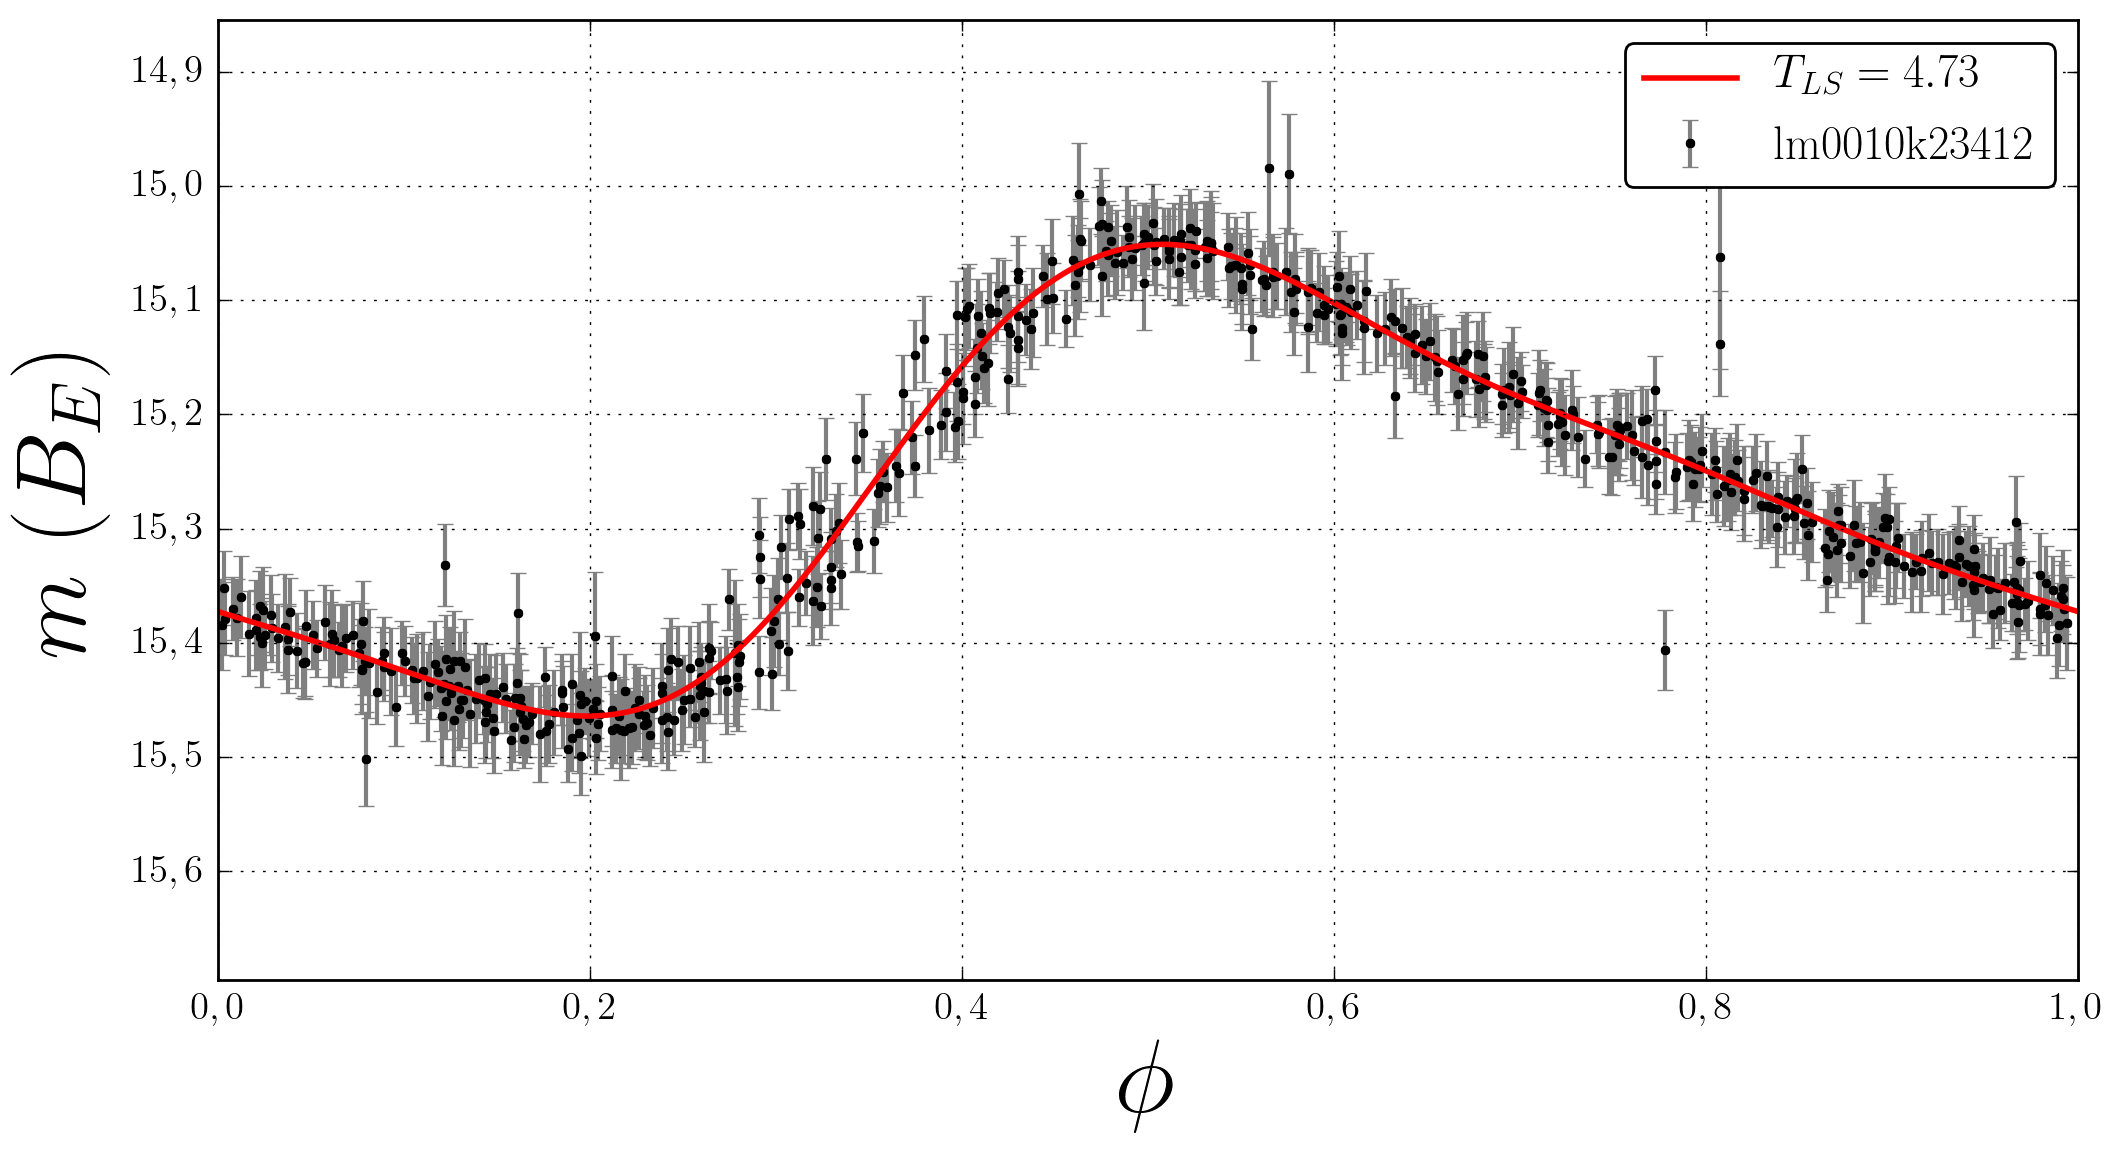
\includegraphics[width=\textwidth]{figures/lightcurves/ceph.png}
	\end{subfigure}
	\begin{subfigure}[t]{0.49\textwidth}
		\centering
		\caption{Type II Cepheid ($T_{\text{LS}} = 12.69 \, \unit{d}$)}
		\label{fig:lightcurve-t2ceph}
		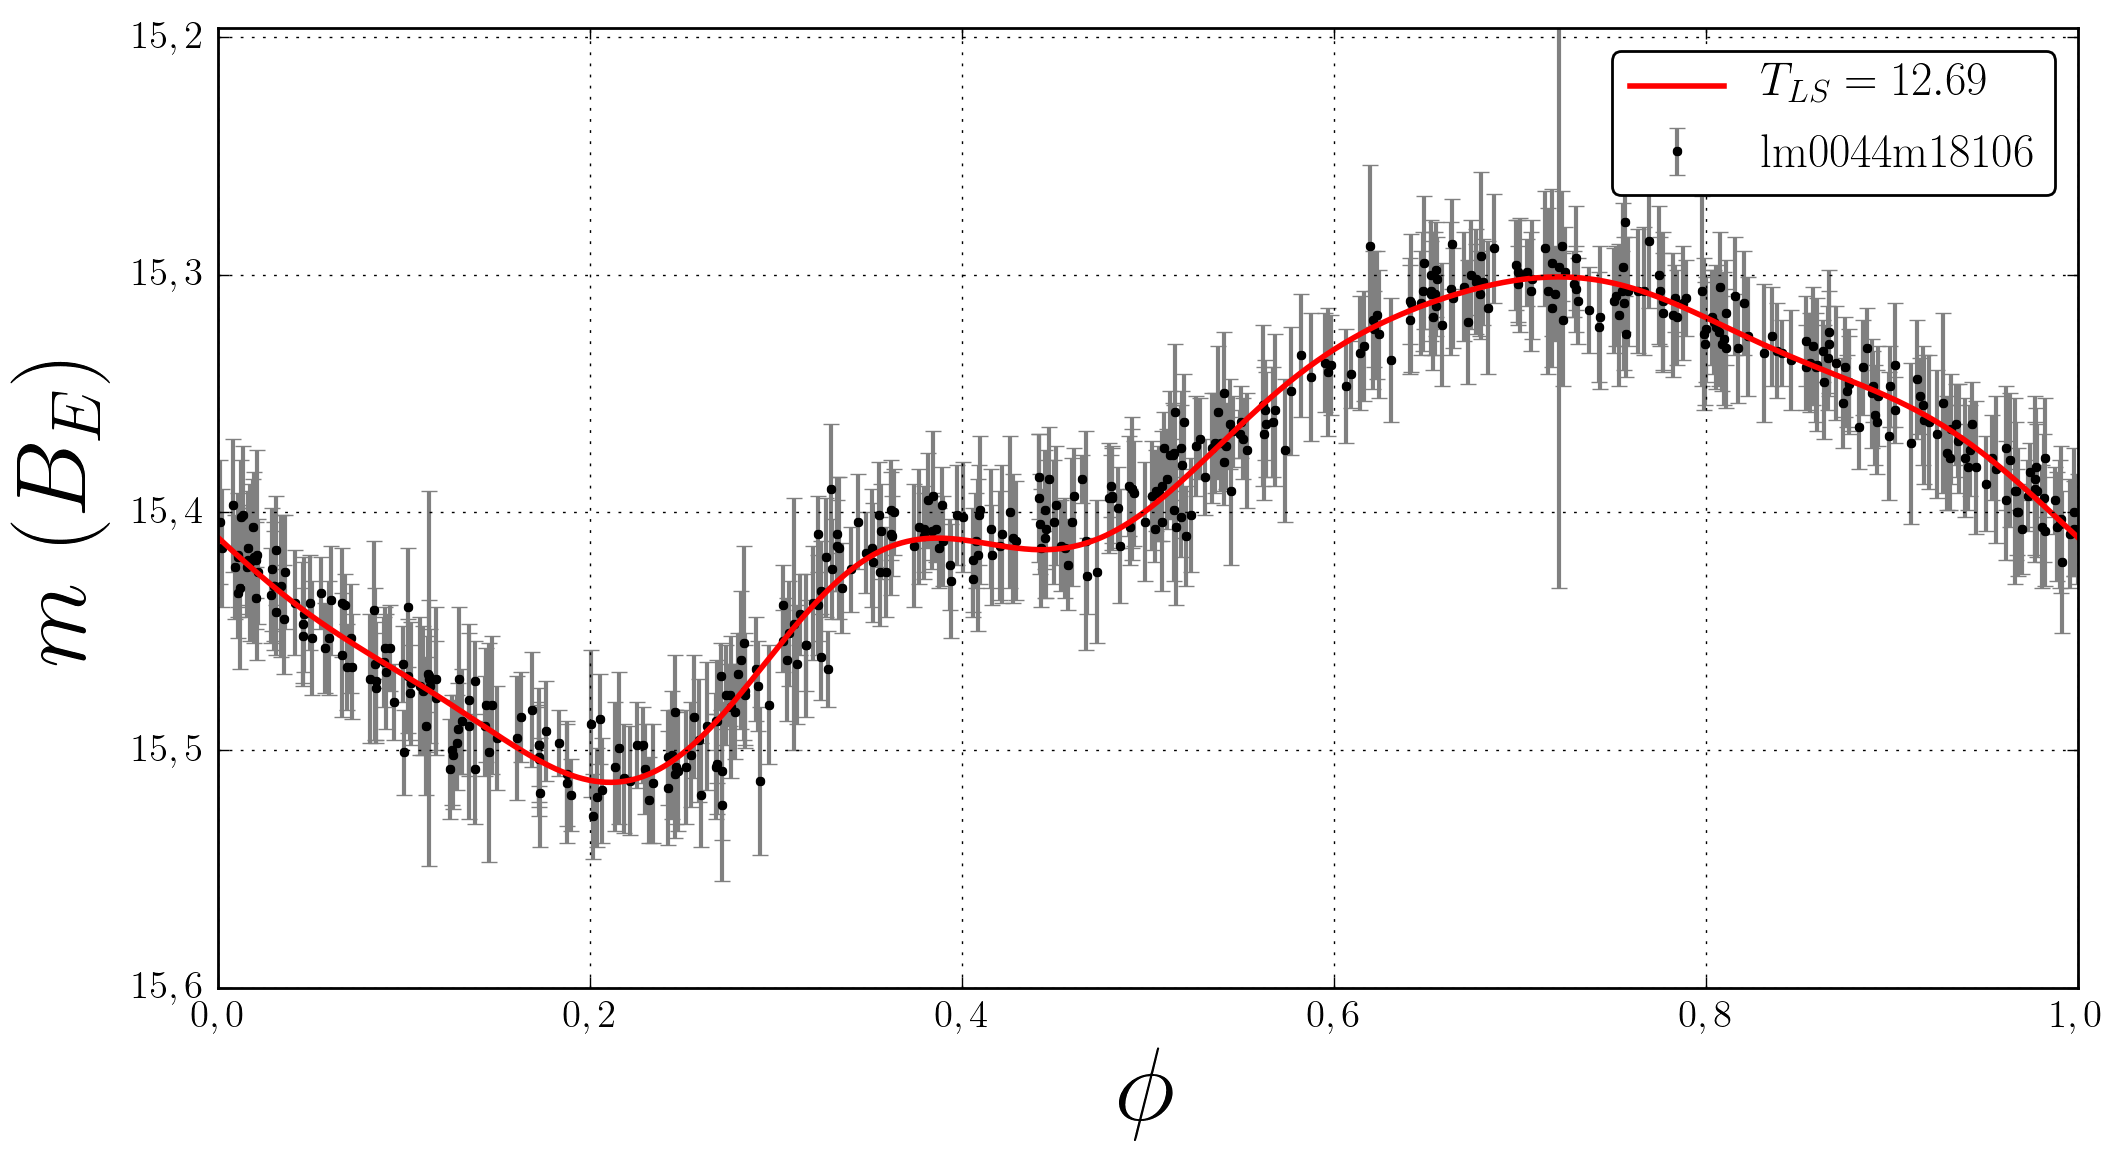
\includegraphics[width=\textwidth]{figures/lightcurves/t2ceph.png}
	\end{subfigure}
	\begin{subfigure}[t]{0.49\textwidth}
		\centering
		\caption{RR Lyrae ($T_{\text{LS}} = 0.51 \, \unit{d}$)}
		\label{fig:lightcurve-rrl}
		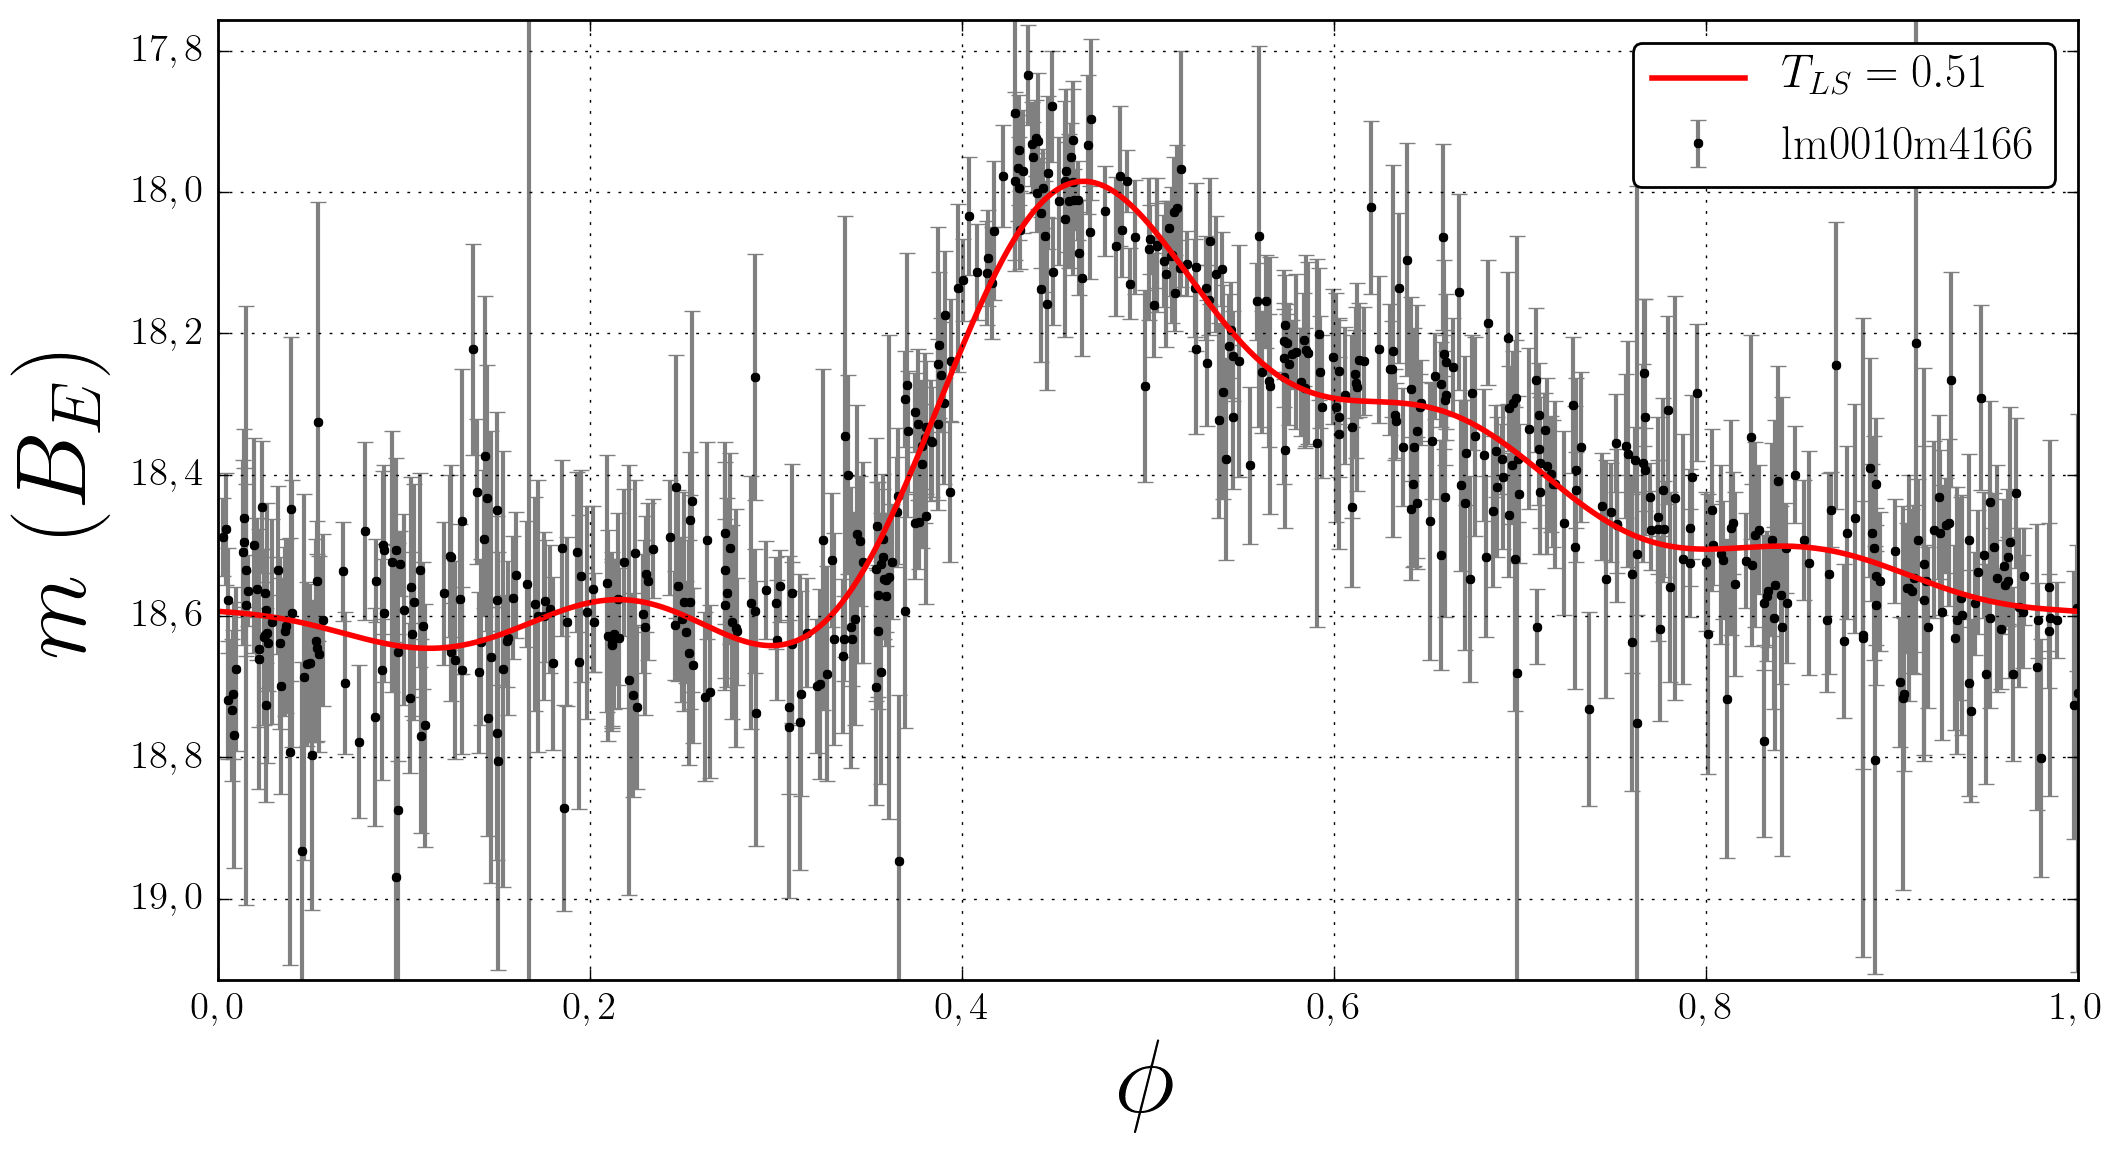
\includegraphics[width=\textwidth]{figures/lightcurves/rrl.png}
	\end{subfigure}
	\begin{subfigure}[t]{0.49\textwidth}
		\centering
		\caption{$\delta$-Scuti ($T_{\text{LS}} = 0.06 \, \unit{d}$)}
		\label{fig:lightcurve-dsct}
		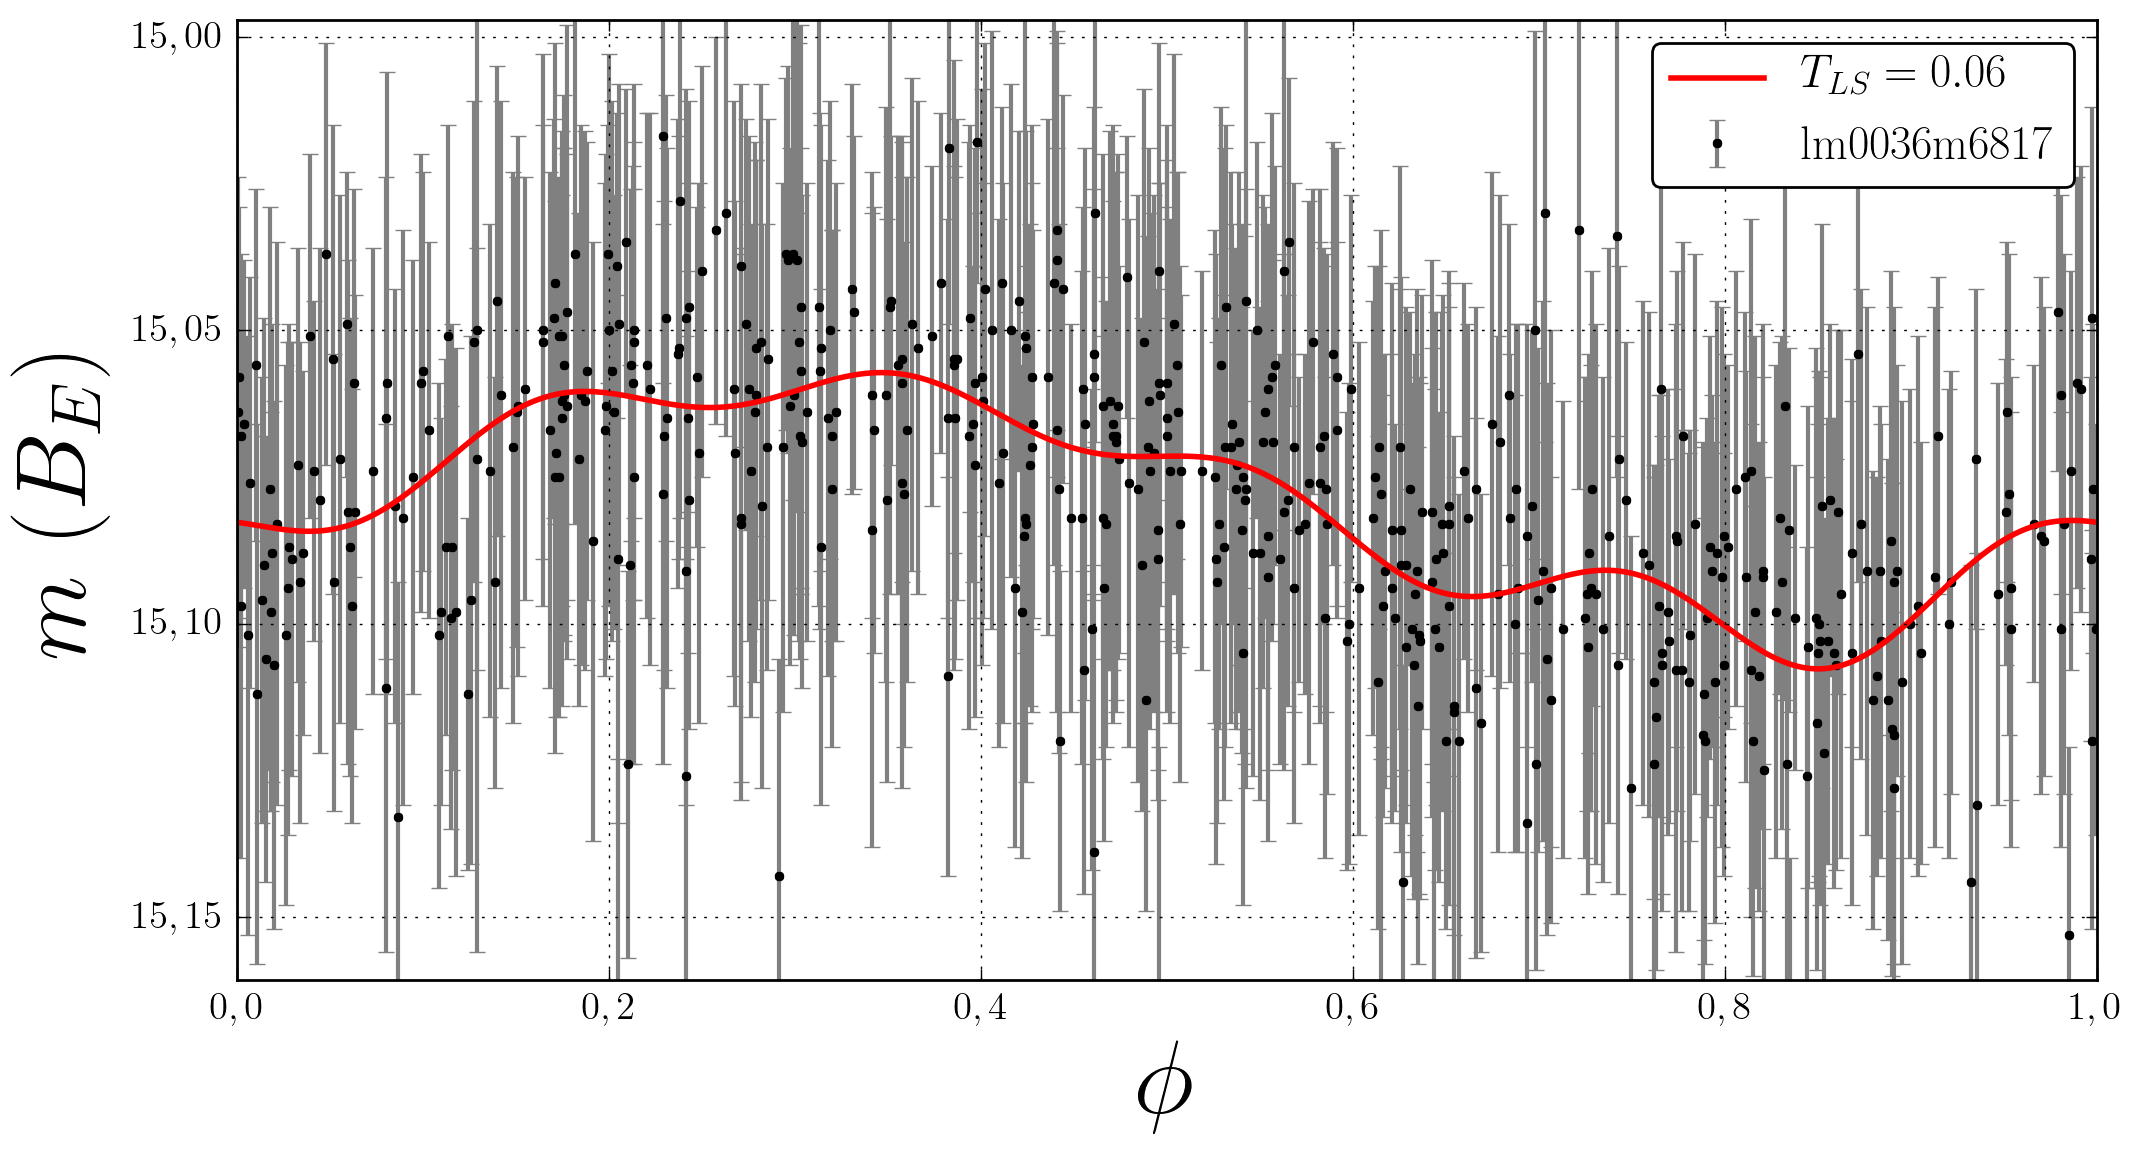
\includegraphics[width=\textwidth]{figures/lightcurves/dsct.png}
	\end{subfigure}
\end{figure}
\begin{figure}[h]
\ContinuedFloat
	\begin{subfigure}[t]{0.49\textwidth}
		\centering
		\caption{Blue variable ($T_{\text{LS}} = 278.57 \, \unit{d}$)}
		\label{fig:lightcurve-bv}
		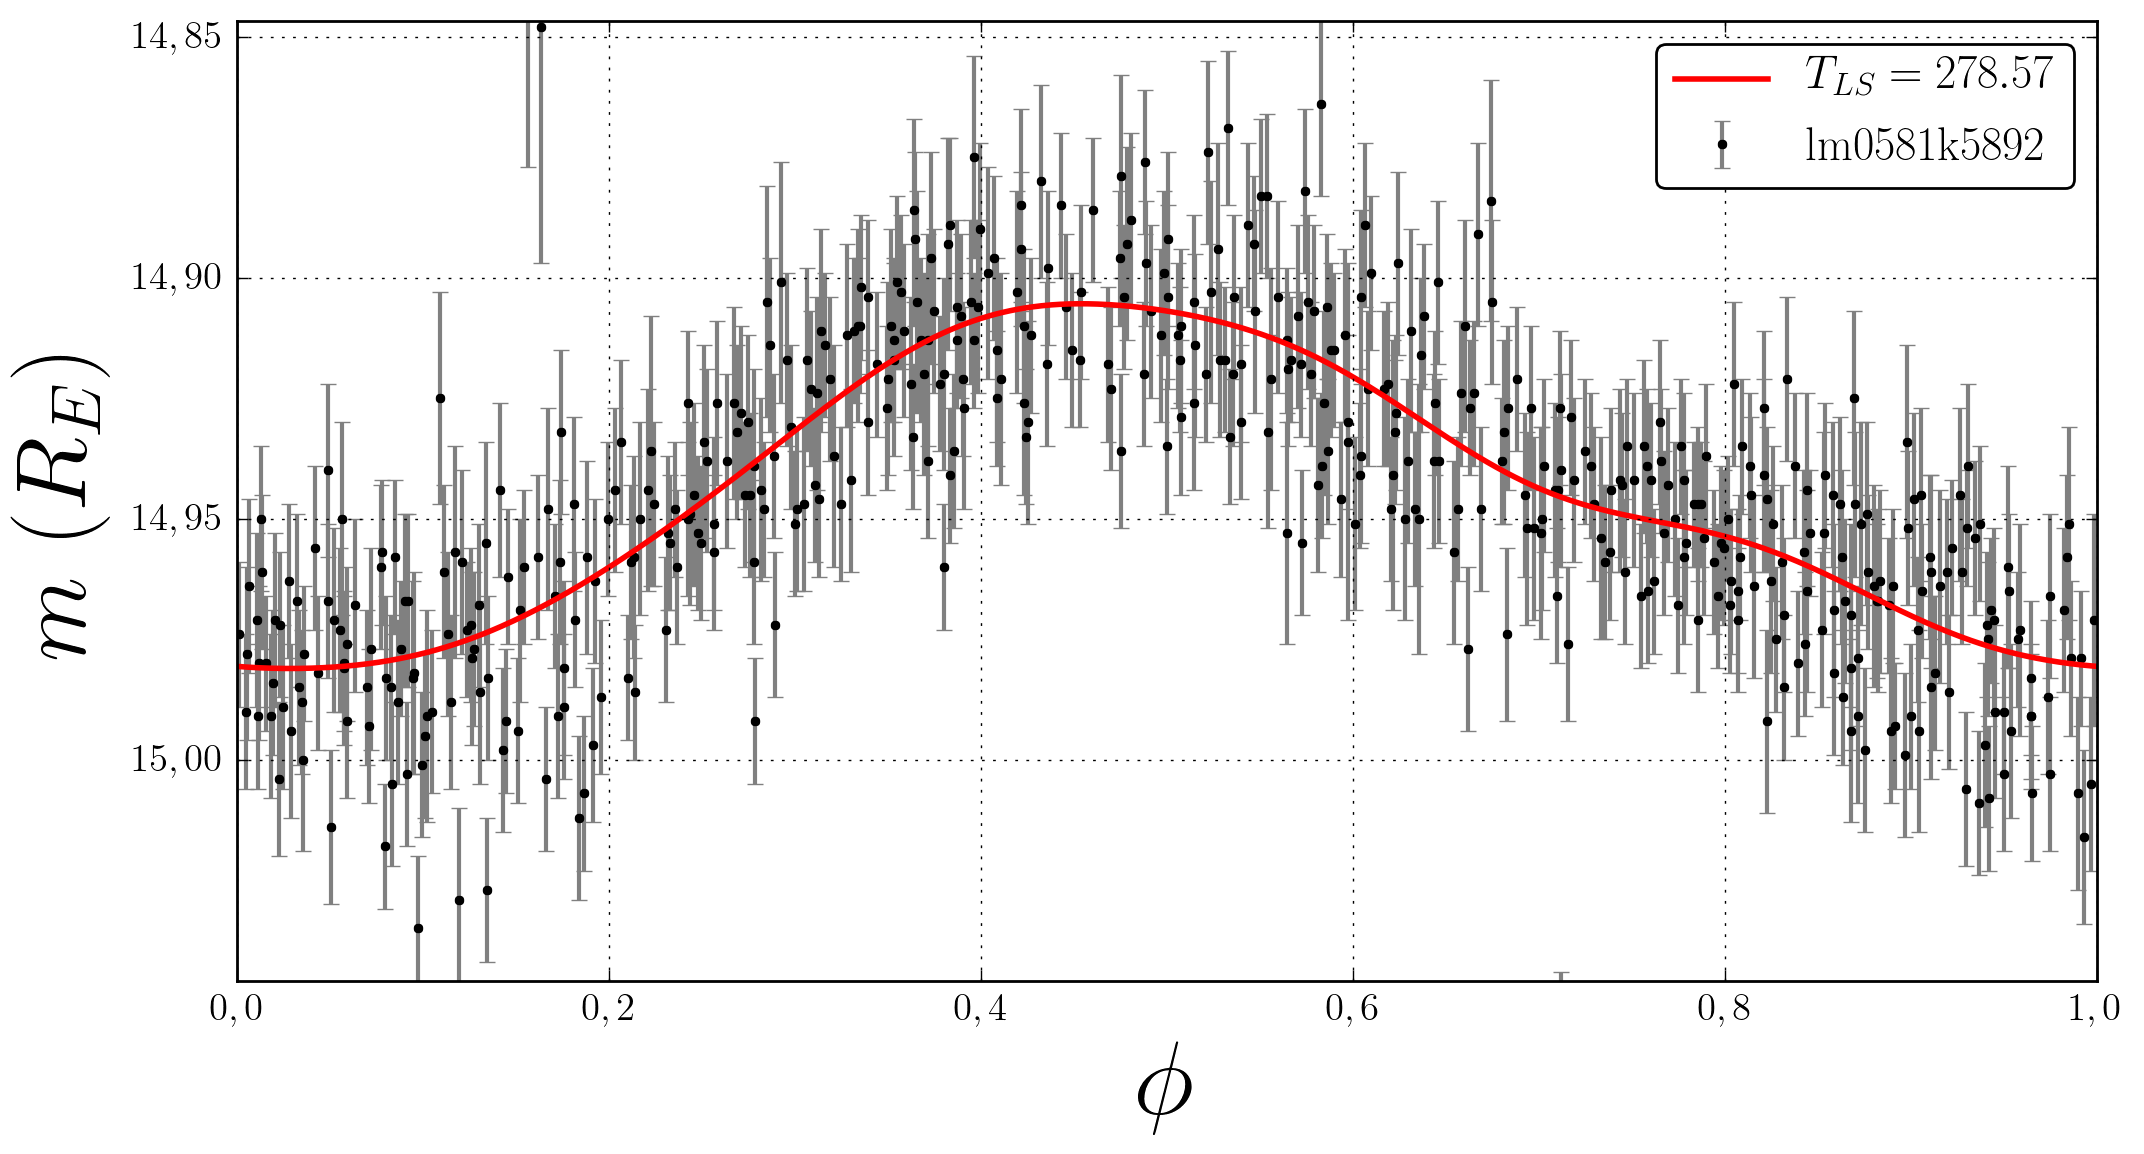
\includegraphics[width=\textwidth]{figures/lightcurves/bv.png}
	\end{subfigure}
	\begin{subfigure}[t]{0.49\textwidth}
		\centering
		\caption{Long--periodic variable ($T_{\text{LS}} = 430.82 \, \unit{d}$)}
		\label{fig:lightcurve-lpv}
		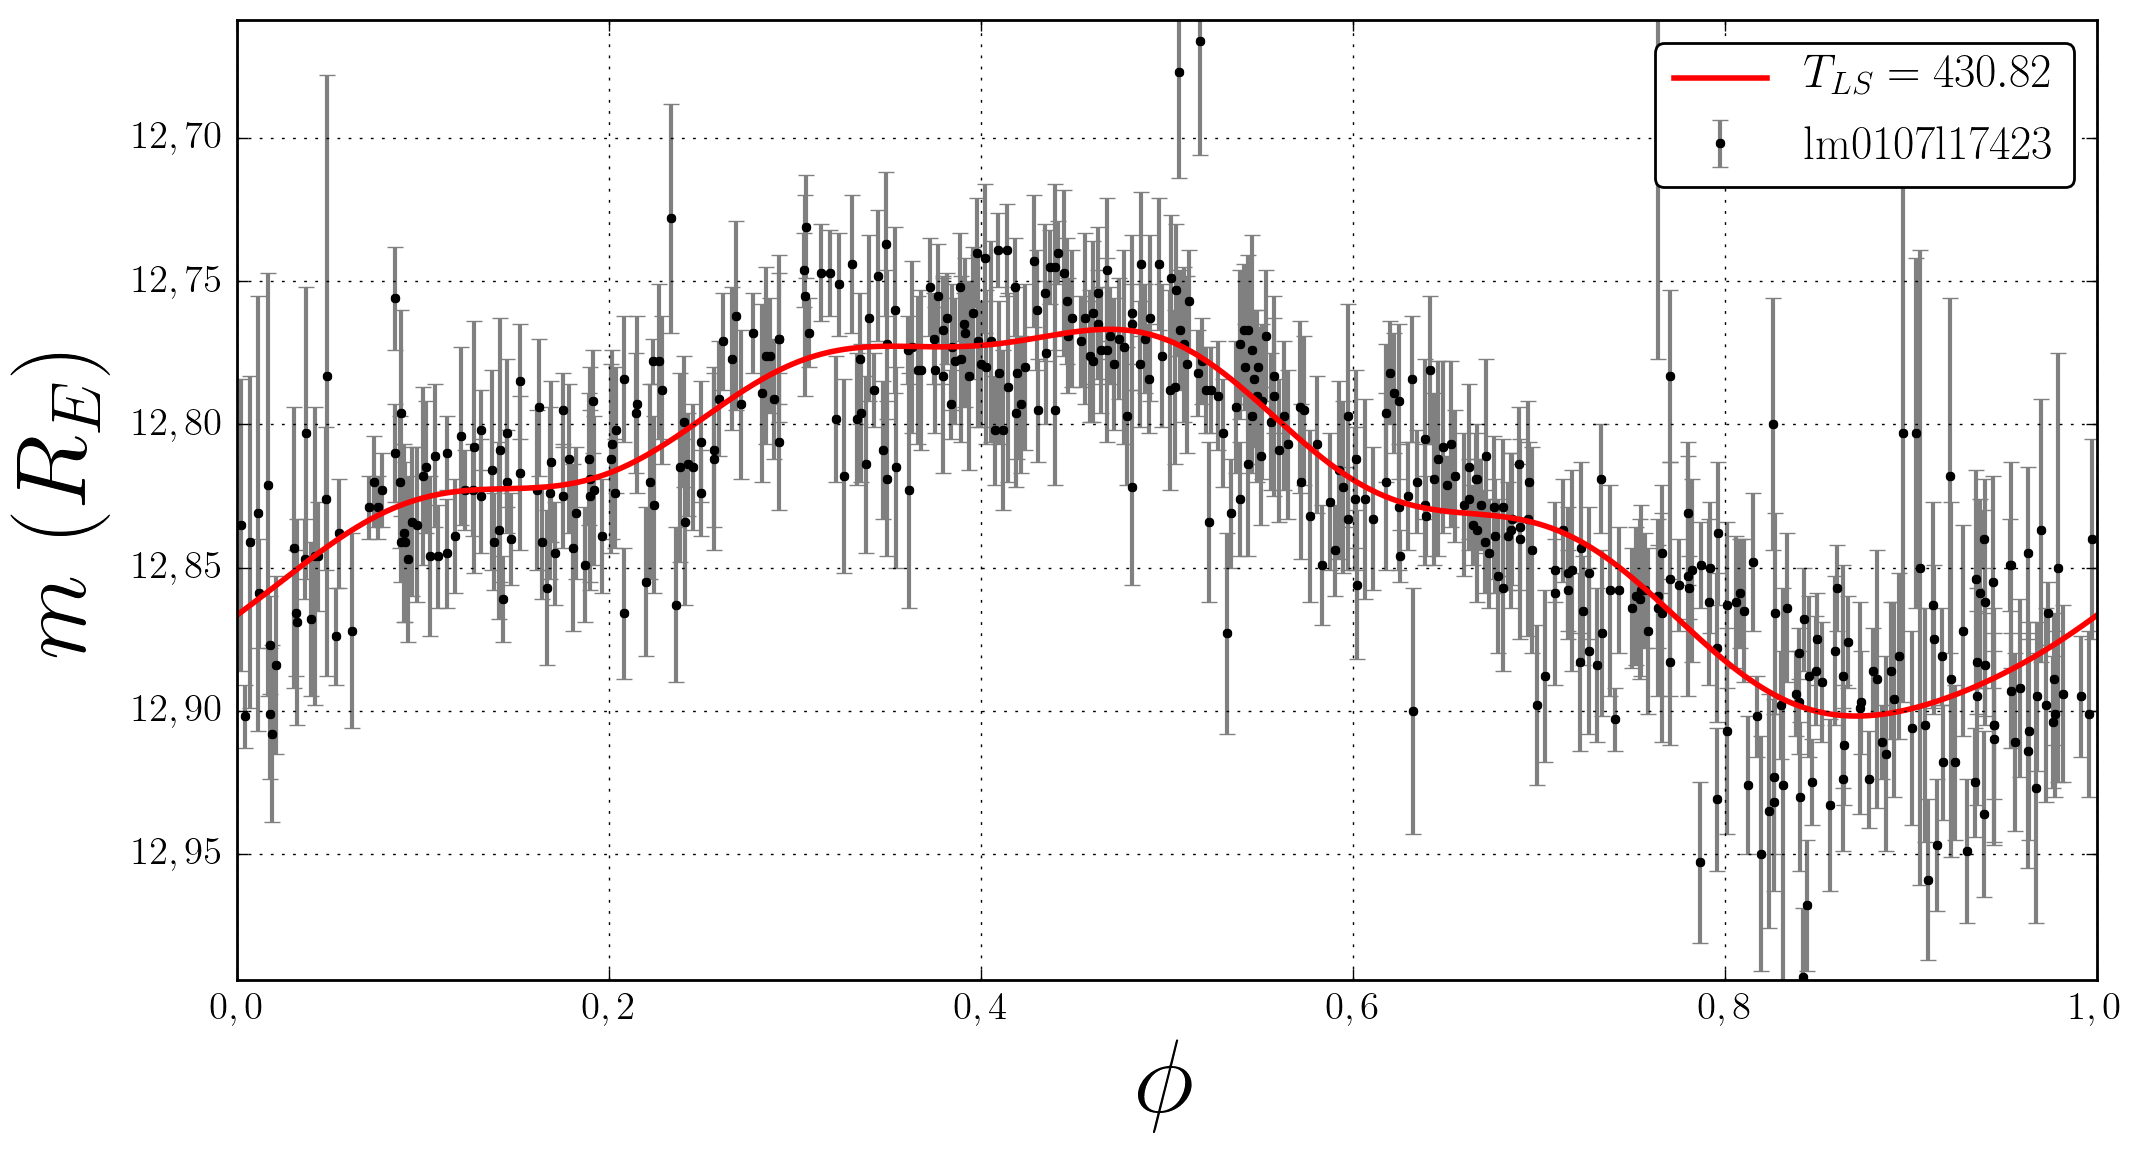
\includegraphics[width=\textwidth]{figures/lightcurves/lpv.png}
	\end{subfigure}
	\begin{subfigure}[t]{0.49\textwidth}
		\centering
		\caption{Eclipsing binary ($T_{\text{LS}} = 0.83 \, \unit{d}$)}
		\label{fig:lightcurve-eb}
		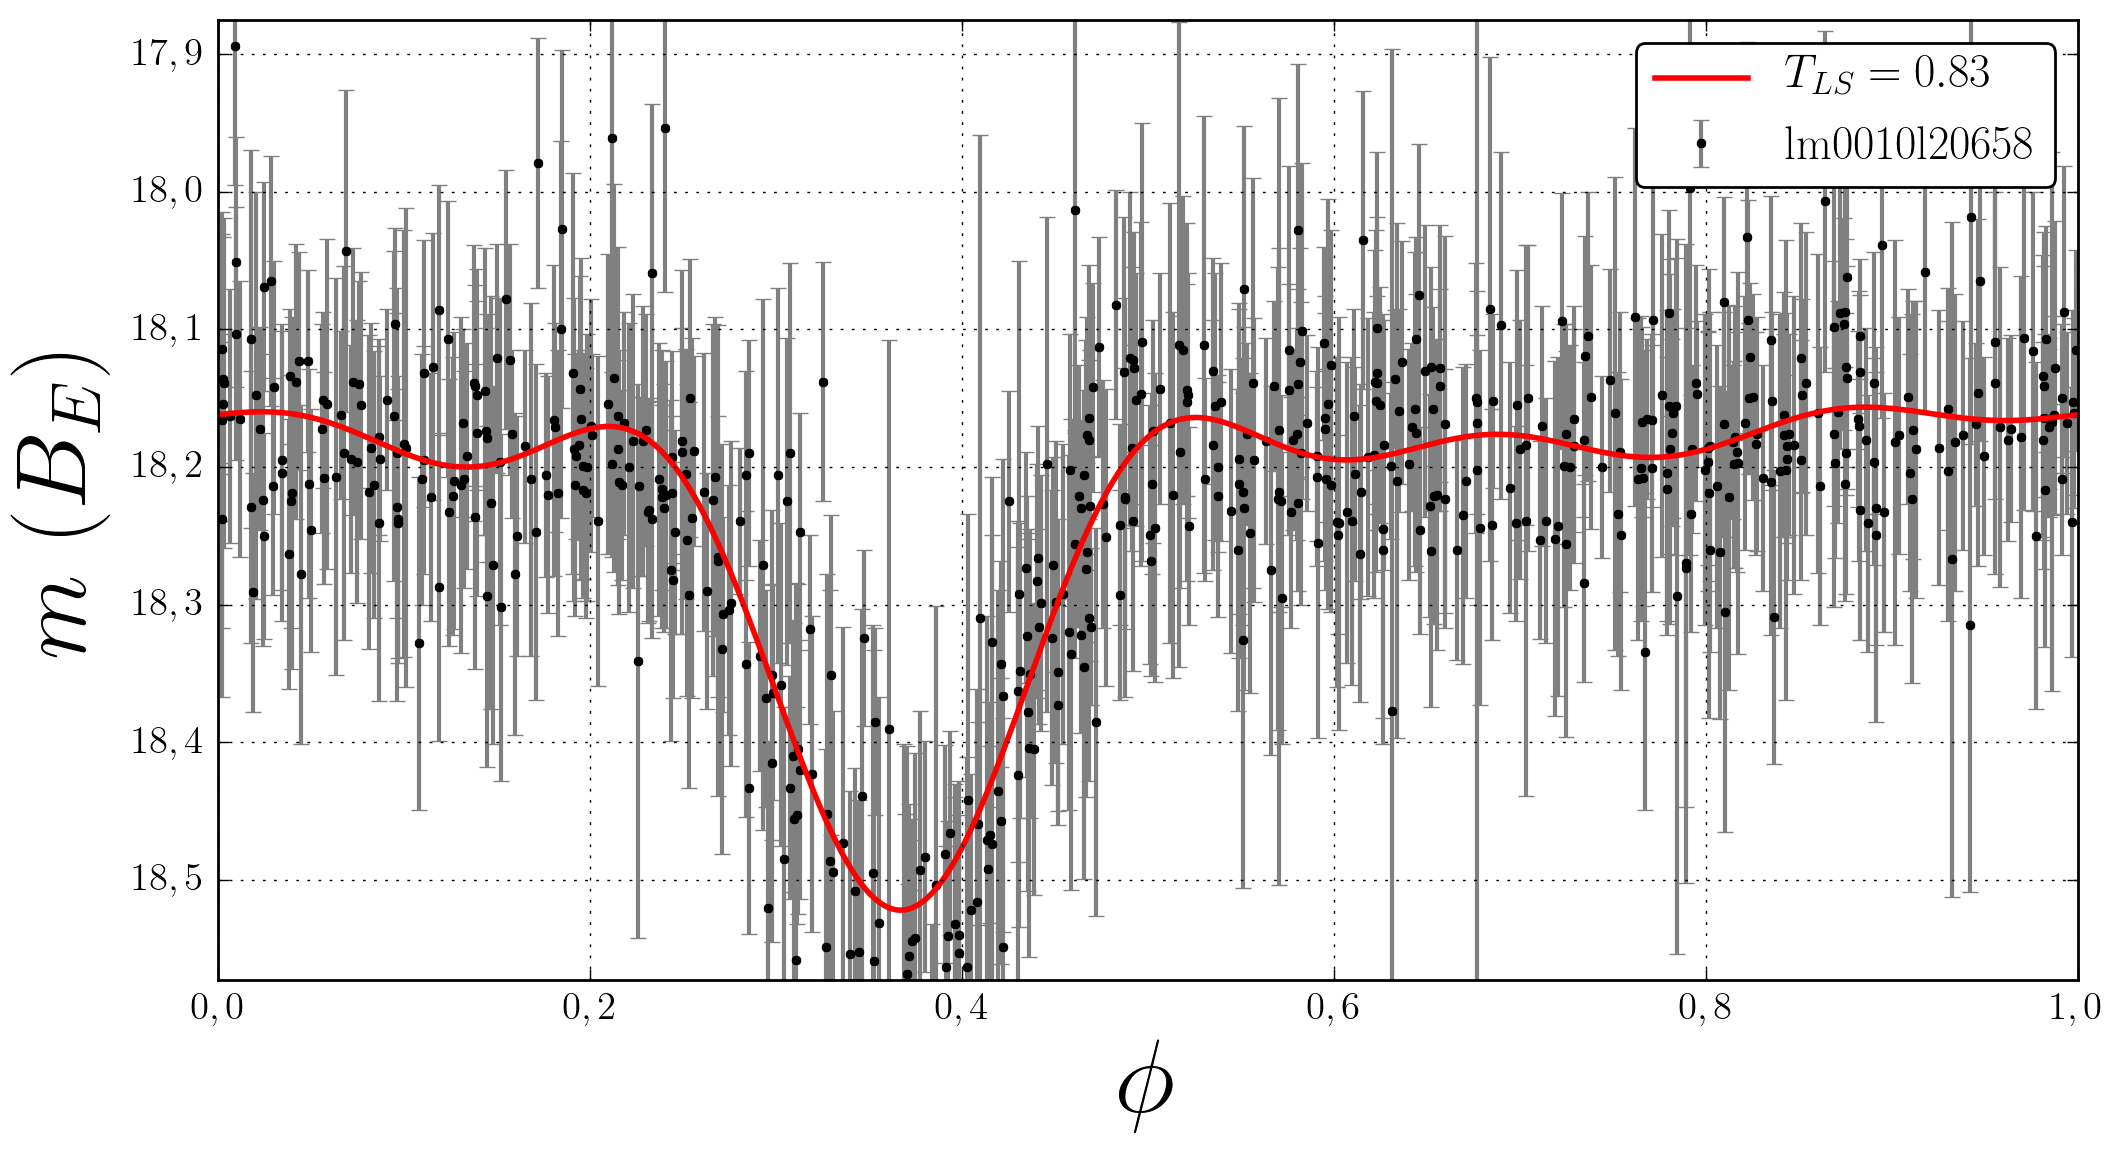
\includegraphics[width=\textwidth]{figures/lightcurves/eb.png}
	\end{subfigure}
	\begin{subfigure}[t]{0.49\textwidth}
		\centering
		\caption{Quasar ($T_{\text{LS}} = 0.05 \, \unit{d}$)}
		\label{fig:lightcurve-qso}
		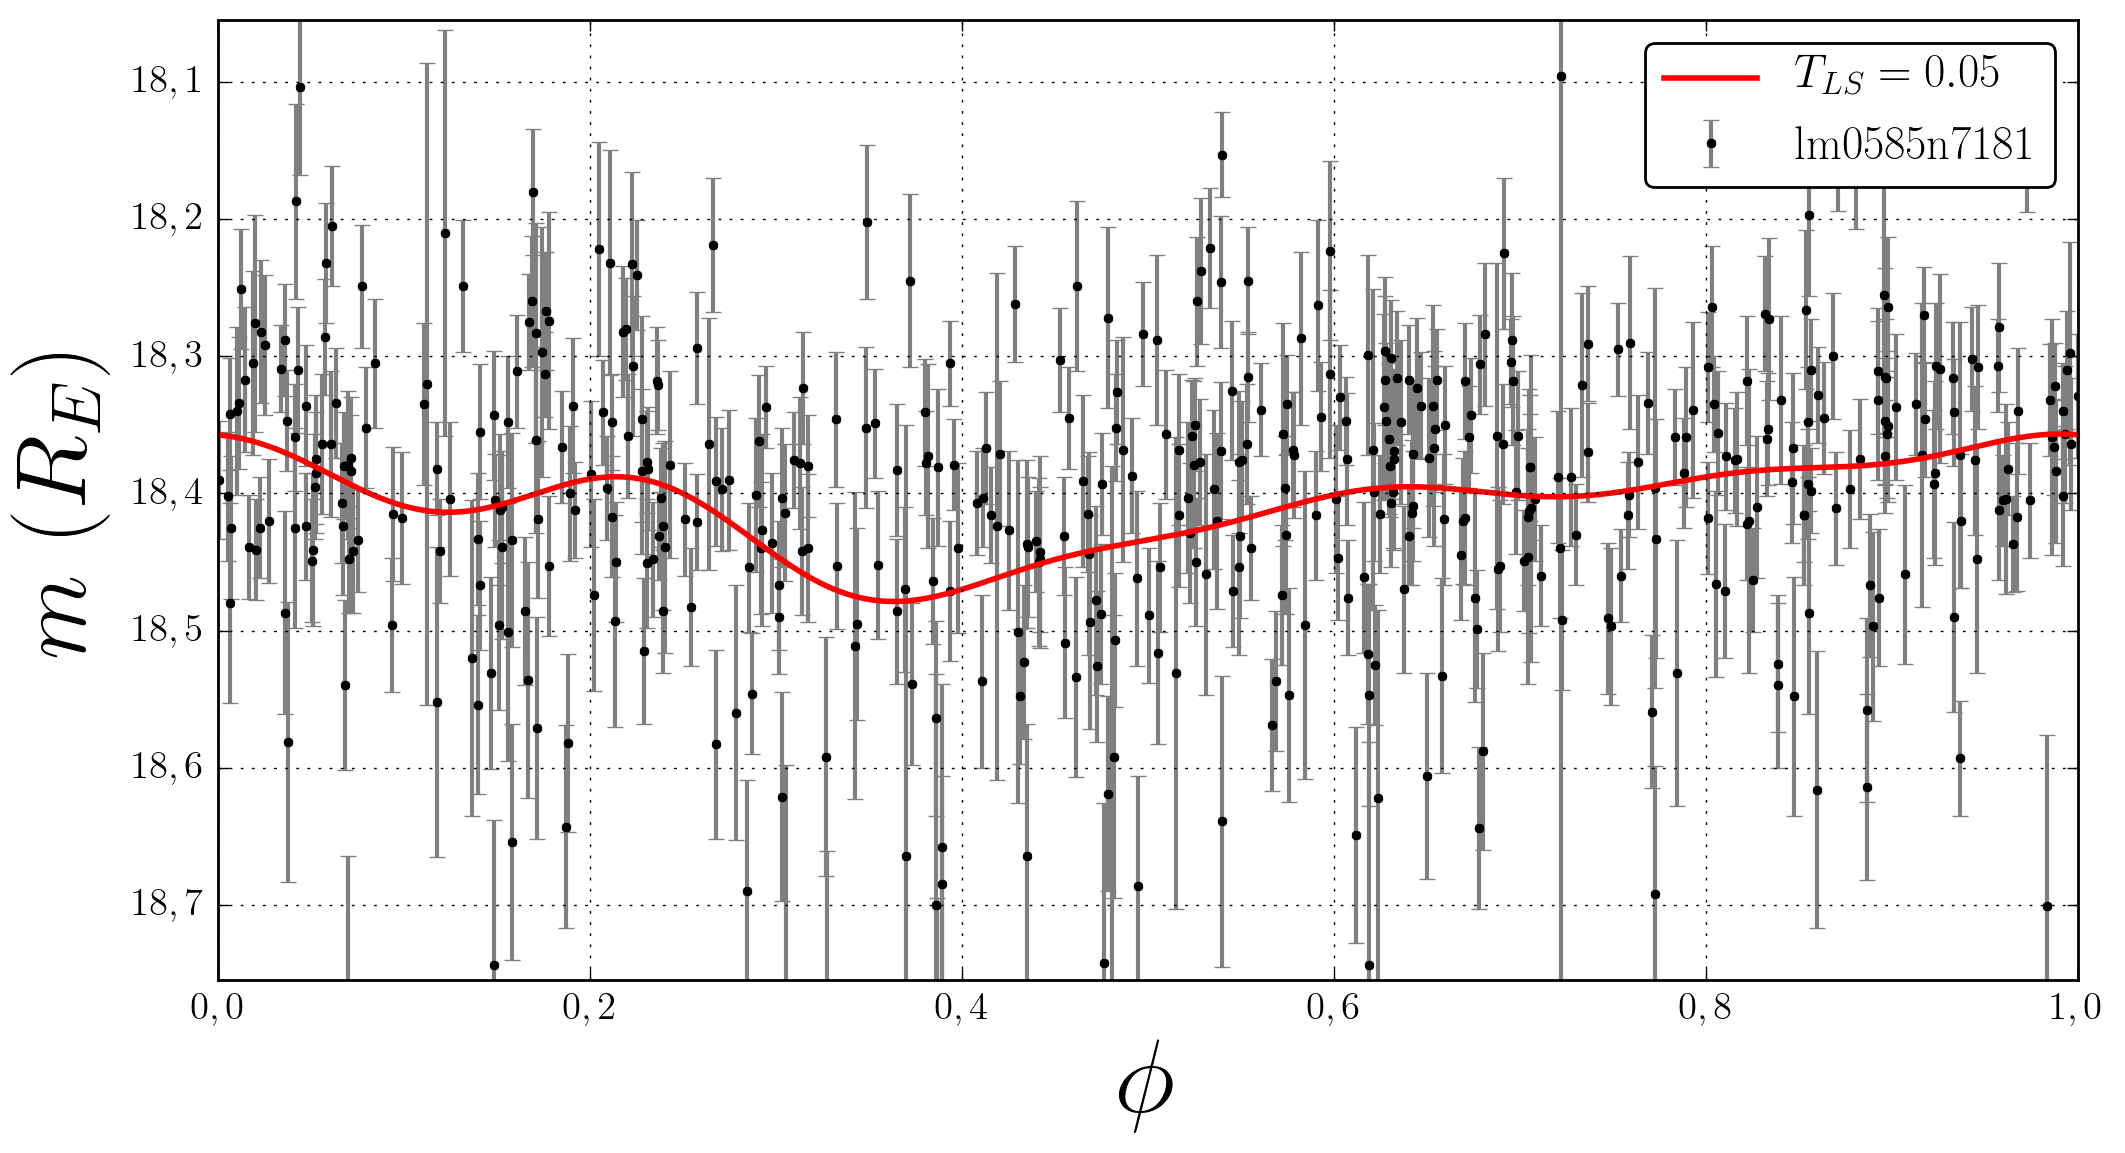
\includegraphics[width=\textwidth]{figures/lightcurves/qso.png}
	\end{subfigure}
	\caption[Light curves for different variable sources]{This figure shows the phase--folded light curves of eight different variables, where the periods were estimated with the Lomb--Scargle algorithm. The red lines indicate a five--term fourier series fit (see equation \eqref{eq:fourier-series-features}). Further comments on the individual light curve shapes can be found in the text.}
	\label{fig:various-light-curves}
\end{figure}

In section \ref{subsec:intrinsic-extrinsic-variability}, we have seen that there are a whole variety of different mechanisms for variability. These mechanisms will lead to distinct light curves, giving rise to discriminative features that can later be used for classification. For the Cepheids (\ref{fig:lightcurve-ceph}), we can see a major change in brightness with small deviations. It is very clear to see that the decline is slower than the incline. The Type II Cepheids (\ref{fig:lightcurve-t2ceph}) show an extra bump in the light curve, which could be caused by a resonance between the different modes \citep{caputo1999}. The RR Lyrae (\ref{fig:lightcurve-rrl}) show a rapid increase followed by a slower decline with some wiggles. The shape is clearly asymmetrical (which is not the case for RRc). $\delta$-Scuti's (\ref{fig:lightcurve-dsct}) light curves are in general similar to Cepheid's or RR Lyrae's, but with a much shorter period. Multi--mode oscillations are very common for $\delta$-Scuti. For the eclipsing binary (\ref{fig:lightcurve-eb}), we can clearly see the expected primary eclipse.

\section{Time Series Analysis}
\label{sec:statistical-analysis-time-series}

When observing one specific object over some time interval $\Delta t$, we can record its magnitude $m_i$ at time $t_i$ and obtain a so-called \emph{light curve}, which is one example of a \emph{time series}. A time series $\Tau$ is a sequence of $N$ data points $(t_i, \vec y_i),\; t_i,(y_i)_j \in \mathbb{R}$ with $t_i < t_{i+1} \; \forall i = 1,\ldots,N$. We call $\Tau$ \emph{evenly--sampled} $\Leftrightarrow t_{i+1} - t_i = C \in \mathbb{R}$ where $C$ is constant. Otherwise, $\Tau$ is \emph{unevenly--sampled}. A time series is called \emph{univariate} if $y_i$ is a scalar, and \emph{multivariate} if $\vec y_i$ is a vector. One example for the latter in astronomy would be the recording of the magnitude for one source at identical $t_i$ in different bands $m_i^{V}, m_i^{R}, m_i^{B}$.\\

Throughout this work, we will often talk about the \emph{phase--fold} of a light curve. This is simply the phase diagram of one complete cycle of the light curve, normalized to be within $[0,1]$, obtained by relocating each point $(t_i, m_i)$ in the time series to its respective position in the cycle,

\begin{equation}
\label{eq:phase-fold}
\phi \colon \mathbb{R} \to \mathbb{R}_{[0, 1]},\, t_i \mapsto \frac{t_i - t_0}{T},
\end{equation}

where $T$ is the period of the signal, and $t_0$ is some arbitrarily selected beginning of the cycle. Figure \ref{fig:unfolded-folded-light-curve} visualizes the difference between both representations of the light curve.\\

\begin{figure}[h]
	\centering
	\begin{subfigure}[t]{0.49\textwidth}
		\centering
		\label{fig:lightcurve-unfolded}
		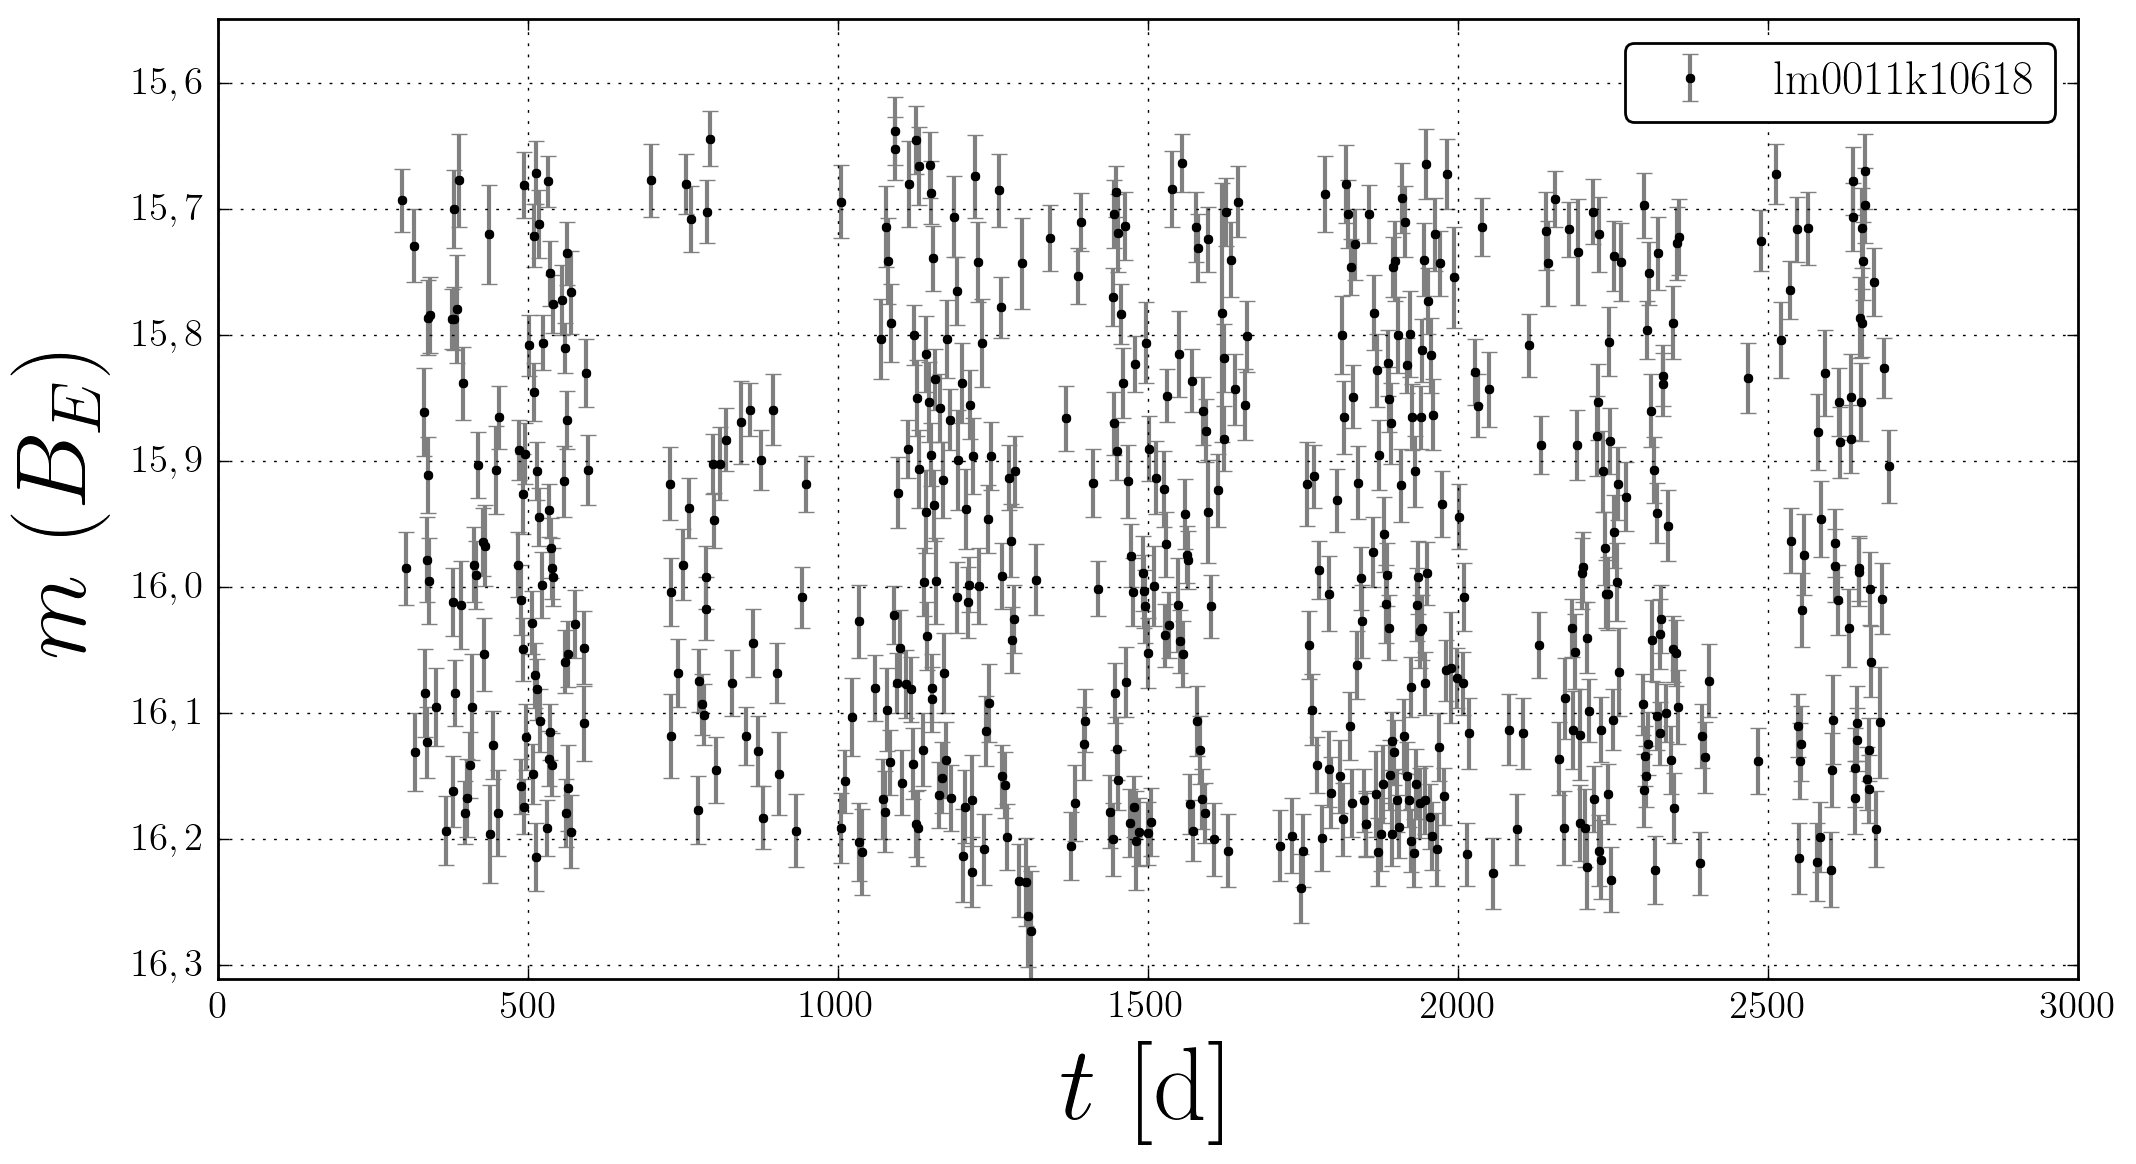
\includegraphics[width=\textwidth]{figures/time-series/lm0011k10618.png}
	\end{subfigure}
	\begin{subfigure}[t]{0.49\textwidth}
		\centering
		\label{fig:lightcurve-folded}
		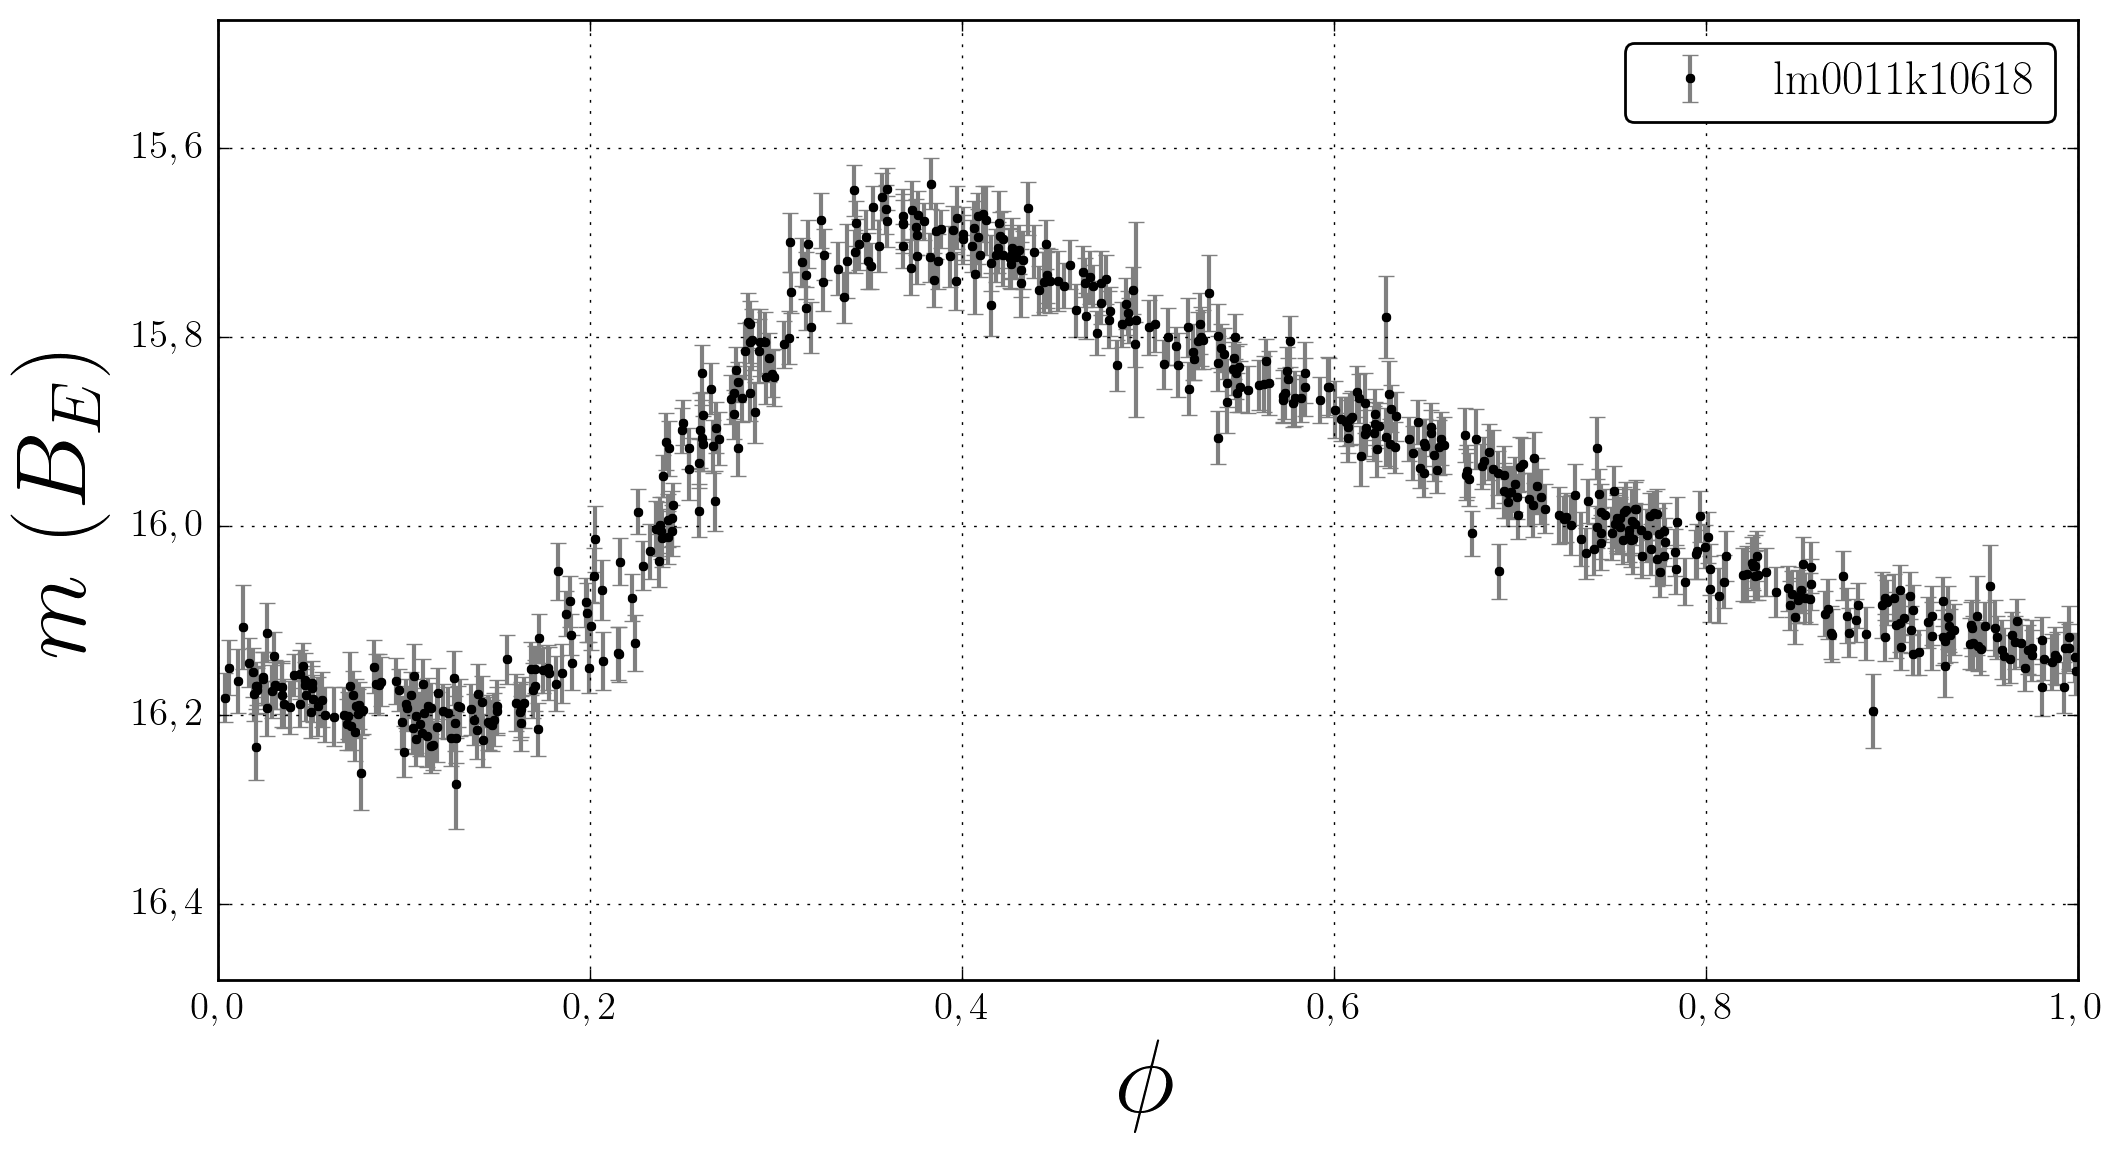
\includegraphics[width=\textwidth]{figures/time-series/lm0011k10618-folded.png}
	\end{subfigure}
	\caption[Raw and phase--folded light curves for EROS ID \emph{lm0011k10618}]{The left panel shows the raw, unfolded light curve of EROS ID \emph{lm0011k10618}. The right panel shows the same light curve, phase--folded with $T_{\text{LS}} = 3.78 \, \unit{d}$. While it is quite hard to infer the type of the source from the left panel, the phase--fold strongly suggests that \emph{lm0011k10618} is a Cepheid.}
	\label{fig:unfolded-folded-light-curve}
\end{figure}

Time series may contain internal structure, \eg by the influence of physical phenomena, or even a superposition of many different effects, which can be recovered by a careful statistical analysis, both in time--domain (auto--correlation and cross--correlation), as well as in frequency--domain (spectral analysis). While there are quite sophisticated methods available for prediction and forecasting, that is, estimating future values based on previous values, \eg by fitting \emph{autoregressive (integrated) moving average} (ARMA/ARIMA) models to the time series, we are merely concerned with signal estimation, \ie separating a meaningful signal from noise and trying to find a model that explains the observation. Specifically, we do this by extracting a variety of \emph{features} from the data, see section \ref{sec:feature-extraction}, which ideally characterize the underlying physics.\\

One very important feature of a periodic signal is, of course, its period $T$. However, reconstructing $T$ from the time series $\Tau$ is not trivial, especially if the data is very noisy. Ultimately, this is a regression problem itself, see subsection \ref{sec:introduction-machine-learning}, however, we will not tackle this with Machine Learning, but rather make use of some well--known methods devised for this very problem.

\subsection{Algorithms for Period-finding}
\label{subsec:period-finding}

Traditionally, most methods available for characterizing a signal in frequency--domain are based on Fourier analysis. They try to find the \emph{periodogram} $P(\omega)$ of signal, which is an estimator for the \emph{spectral density} $P$ as a function of the angular frequency $\omega = \frac{2 \pi}{T}$\footnote{In this regard, the periodogram can be seen as spectrum (some quantity over frequency) of a time series $\Tau$.}. In 1898, Arthur Schuster defined the \emph{Schuster periodogram}

\begin{equation}
\label{eg:schuster-periodogram}
P_{\text{S}}(\omega) = \frac{1}{k} \, \biggl| \, \sum\limits_{i=1}^{k} y_i \, \euler^{-\mathrm{i} \omega t_i} \, \biggr|^2,
\end{equation}

% If omega0 is true period than e^{-i * omega0 * t_i} will have large contribution
% https://charlesmartin14.wordpress.com/2012/11/05/noisy-time-series/
% Reference for Schuster periodogram

for a time series $(t_i, y_i)$ of length $k$. Note that equation \eqref{eg:schuster-periodogram} is essentially given by $\| \mathcal{F}(\omega) \|_2 $, the $L^2$ norm of the discrete Fourier transform (DFT) $\mathcal{F}$ of the signal. Therefore, $P_{\text{S}}(\omega)$ can be approximated very efficiently by using the fast Fourier transform algorithm (FFT) \citep{cooley1965}, which allows for a runtime complexity of $\mathcal{O}(N\log{(N)})$ instead of $\mathcal{O}(N^2)$. However, it can be shown that those Fourier transform--based methods perform poorly on unevenly--sampled data, because they tend to boost long--periodic noise in the periodogram \citep{hastie2001}. Since evenly--sampled data can be difficult to obtain, especially for earth--bound surveys in astronomy, a lot of effort was put into developing suitable methods that can cope with this kind of data. This work makes use of two popular methods devised for unevenly--sampled data, one based on least--squares spectral analysis (LSSA), namely the \emph{Lomb--Scargle periodogram}, and the other one based on the minimization of some metric for dispersion in phase space, in this case \emph{conditional entropy}. We provide a brief overview for both of them.

\subsubsection{Lomb--Scargle Periodogram}
\label{subsubsec:lomb-scargle}

The most prominent method for finding the period of an unevenly--sampled light curve was developed by \citet{lomb1976} and extended by \citet{scargle1982}. It is devised to find the period of a sinusoidal--shaped periodic signal. For a given time--series $(t_i, (y_i, \sigma_i))$ of length $k$ with arithmetic mean $\mu_y$ and variance of the noise $\sigma_y^2$, Scargle defines the \emph{normalized Lomb--Scargle periodogram} as

\begin{equation}
\label{eq:normalized-lomb-scargle}
P^{\text{N}}_{\text{LS}}(\omega) = \frac{1}{2 \sigma_y^2} \Bigg\{ \frac{\big[\sum\limits_{i=1}^k (y_i - \mu_y) \cos(\omega(t_i - \tau))\big]^2}{\sum\limits_{i=1}^k \cos^2(\omega(t_i - \tau))} + \frac{\big[\sum\limits_{i=1}^k (y_i - \mu_y) \sin(\omega(t_i - \tau))\big]^2}{\sum\limits_{i=1}^k \sin^2(\omega(t_i - \tau))}\Bigg\},
\end{equation}

where $\tau$ is a time--offset defined by

\begin{equation}
\tan(2 \omega \tau) = \frac{\sum\limits_{i=1}^k \sin(2 \omega t_i)}{\sum\limits_{i=1}^k \cos(2 \omega t_i)},
\end{equation}

which makes the periodogram $P^{\text{N}}_{\text{LS}}(\omega)$ invariant for a translation in $t$. Furthermore, this time--offset $\tau$ makes the periodogram identical to least--squares fitting of a single--component sinusoidal model of the form $y(t) = A \sin(\omega t + \varphi)$ \citep{horne1986, vanderplas2015}. Additionally it can be shown that --- if the periodogram is properly normalized\footnote{There has been a lively discussion about the correct normalization of the periodogram, which retains above convenient statistical properties, see \citet{lomb1976,astroML,zechmeister2009}. The correct normalization factor in equation \eqref{eq:normalized-lomb-scargle} is \emph{the total variance of the data}, as explained in detail in \citet{horne1986}.} --- $P^{\text{N}}_{\text{LS}}(\omega_0) \propto \exp(-x)$ for pure noise at any frequency $\omega_0$, where $x$ denotes the height of the peak. This exponential probability distribution gives rise to the \emph{false--alarm probability (FAP)},

\begin{equation}
\text{FAP}_{\text{LS}}(x) = 1 - (1 - \euler^{-x})^M,
\end{equation}

which is a suitable and convenient estimator for the significance\footnote{In this case: The probability that the peak is the product of a true signal, rather than the result of randomly distributed noise.} of a peak. It quantifies the probability that a peak of at least height $x$ will occur in a periodogram on a grid of $M$ independent frequencies \emph{when evaluated on pure noise} \citep{horne1986}.\\

In spite of its usefulness, there are some drawbacks of the normalized Lomb--Scargle periodogram in its original formulation:

\begin{itemize}
\item $P^{\text{N}}_{\text{LS}}(\omega)$ given by equation \eqref{eq:normalized-lomb-scargle} does not account for measurement errors, \eg by introducing weights for all data points. This however ignores an important aspect of the measurement process, where some data points might in fact be more accurate than others, for example due to changing conditions in the measurement environment.
\item In \eqref{eq:normalized-lomb-scargle} we substract the mean of the data $\mu_y$ from $y_i$ which assumes that the mean of the underlying sine wave and the observed data are identical \citep{cumming1999}. This assumption might not always hold, \eg for unfortunate sampling cadence or in the case of very few data points, where $\mu_y$ is not a robust estimate of the signal's true mean.
\end{itemize}

To overcome these limitations, \citeauthor{zechmeister2009} have introduced the \emph{Generalized Lomb--Scargle periodogram} which essentially generalizes the original formulation towards $\chi^2$ fitting of a full sine wave including an offset. The details, including an analytic solution, are described in \citet{zechmeister2009}.

% This led to further generalization...
% The \emph{generalized Lomb--Scargle periodogram} is less prone to aliasing, and provides more accurate results (http://arxiv.org/abs/0901.2573).

% Generalized and classical
% Bayesian generalized Lomb-Scargle (Martiniee)
% Single point estimate rather than a posterior probability distribution
% Multi-band periodogram and matrix formalism
% It is possible to carefully correct for such aliasing by iteratively removing contributions from the estimated window function (e.g. Roberts et al.1987), we’ll ignore this detail in the current work.
% Discrete and continous, Fast Fourier Transformation (FFT)
% Remarks concerning runtime N^2 and Nlog(N) implementations

\subsubsection{Conditional Entropy Periodogram}
\label{subsubsec:conditional-entropy}

Using conditional entropy for period finding was first proposed by \citet{graham2013} as an extension of a similar algorithm developed by \citet{cincotta1995}. Both algorithms look at the problem from an information--theoretic point of view, which makes them interesting for us because this is fundamentally different to the Lomb--Scargle aglorithm. The fundamental idea is that the phase--folded light curve will form the most ordered, compact arrangement of points in phase space when folded with the true period, whereas it would look very noisy for most other periods. One way to quantify this would be to partition the normalized $m$-$\phi$-square into $k$ bins for each candidate period $\hat T_i$, and then calculating the \emph{Shannon entropy}

\begin{equation}
\label{eq:shannon-entropy}
E_\text{S} = - \sum_{i=1}^k \mu_i \ln(\mu_i),
\end{equation}

where $\mu_i = \frac{n_i}{N}$ denotes the occupation probability for the $i^\text{th}$ bin, which is simply the number of data points in the $i^\text{th}$ bin $n_i$ over the total number of data points $N$. The best estimate of the true period $T$ would then be the candidate period $\hat T_i$ which minimizes equation \eqref{eq:shannon-entropy}. It has been established that this does not yield satisfying results on real--world data \citep{cincotta1999}, because the resulting periods are very often corresponding to the mean solar day $T_{\text{Solar}} = 1.00274 \, \unit{d}$. This effect can be corrected for to some extent, \eg by a wise choice of the partitioning as described by \citet{cincotta1999} and \citet{drake2013}. For this reason \citeauthor{graham2013} devised their enhancement by proposing to substitute equation \eqref{eq:shannon-entropy} with the \emph{conditional entropy}

\begin{equation}
E_\text{CE} = \sum_{i,j} \mu(m_i, \phi_i) \ln\big(\frac{\mu(\phi_j)}{\mu(m_i, \phi_j)}\big),
\end{equation}

where $\mu(m_i, \phi_i)$ denotes the occupation probability for the $i^\text{th}$ partition in magnitude within the $j^\text{th}$ partition in phase.\\

\subsection{Structure Function \& Stochastic Variability}
\label{subsec:structure-function}

As we have seen in section \ref{sec:theory-variable-objects}, quasars change their luminosity in a chaotic, stochastic manner. The precise physical cause for this variability is subject to ongoing research. \citet{pereyra2006} and \citet{li2008} present evidence that the variability is caused by a variable accretion rate $\dot M$. On the other hand, \citet{blackburne2010} demonstrate that a change in the effective area of the accretion disk could contribute to the overall variability. Regardless of the actual cause, QSO observations, \eg light curves, can be described in a statistical manner. Structure function $\text{SF}$ analysis \citep{hughes1992,collier2001} is one way to do this, and has been shown (\eg \citet{schmidt2010}) to provide robust results in separating quasars from other variable sources. It characterizes the intrinsic, stochastic variability of a source by quantifying the variability amplitude $V$ of an object as a function of the time lag $\Delta t_{ij}$ between two observations $m_i, m_j$. This can be done for a large ensemble of sources, to analyse the properties of an entire population, or, if proper sampling is available, for individual objects. Given a magnitude time series of length $N$, we build a list of the $\frac{N(N-1)}{2}$ data pairs, and estimate the variability by

\begin{equation}
V_{ij}(\Delta t_{ij}) = \Delta m_{ij} - \sqrt{\sigma_i + \sigma_j},
\end{equation}

where the last term corrects for the photometric measurement errors, and $\Delta m_{ij}$ is the magnitude difference $m_i - m_j$. It is important to note that $\Delta t_{ij}$ denotes the time lag in the observed frame and \emph{not} in the object's rest frame. In principle, we could correct for this if further knowledge about the object's red shift was available. We then define the binned structure function as

\begin{equation}
\text{SF}(\Delta t) = \big\langle \sqrt{\frac{\pi}{2}} \big| \Delta m_{ij}  \big| - \sqrt{\sigma_{m_i}^2 + \sigma_{m_j}^2} \big\rangle_{\Delta \tau},
\label{eq:binned-structure-function}
\end{equation}

where $\langle \cdot \rangle_{\Delta \tau}$ is the arithmetic mean of all data points within bin $\Delta \tau$.\footnote{There are a lot of different definitions of equation \eqref{eq:binned-structure-function}. We decide to follow \citet{schmidt2010}.} It has been established \citep{richards2006} that a power--law model of the form

\begin{equation}
A \, \big(\frac{\Delta t}{1 \, \unit{yr}}\big)^\gamma
\end{equation}

provides a decent fit for \eqref{eq:binned-structure-function}, where $A$ is an estimate of the root--mean--square magnitude variability on the timescale of $1 \, \unit{yr}$ and $\gamma$ is the logarithmic gradient of the change in magnitude. As described in section \ref{sec:feature-extraction}, we fit this model using linear optimization and add the two parameters as features for the light curves.

\section{Statistical Inference Using Machine Learning}

\subsection{Introduction to Machine Learning}
\label{sec:introduction-machine-learning}

\emph{Machine Learning} (ML), sometimes referred to as \emph{pattern recognition}, is a subfield of Artificial Intelligence (AI) primarily dealing with automated approaches to infer meaning from data. Depending on the problem to be solved and the data available, Machine Learning algorithms can be divided into \emph{supervised}, \emph{unsupervised} and \emph{reinforcement} learning. In supervised learning, we provide examples of the desired output to a model in such a way that, after some training process, a model is obtained, that can later be used to make predictions or decisions on similar data. This is a form of learning, because rather than explicitly programming certain decision rules, we want to generalize observations towards an underlying model that performs as well as possible when confronted with new data. Typical supervised learning tasks are \emph{classification problems} and \emph{regression problems}. Unsupervised learning however tries to discover internal structure in the data, \eg searching for clusters in feature space (\emph{clustering}), \emph{density estimation} or finding a lower--dimensional representation of the data by means of \emph{dimensionality reduction}. Reinforcement learning refers to a setting where a software agent has to take decisions based on the current state of the system under the constant feedback from the environment, trying to maximize some cumulative \emph{reward} function.\\

% In the context of model evaluation, \emph{overfitting} describes a scenario where an overly complex model fits noise instead of ...

In consideration of the fact that generalization is of utter importance to predictive modelling, we have to take adequate provisions to avoid bad performance on unseen data. Otherwise we can not justify the assumption that our model will be able to cope with new data, leaving us with a more or less useless model of reality\footnote{In fact, this becomes even worse when people or machines blindly believe in our model, making decisions based on our predictions, which are in fact systematically wrong.}. For this reason, we \emph{thoroughly} separate training and testing data throughout the process of model fitting. One way to do this kind of model validation is \emph{cross--validation}. This work makes use of $k$--fold cross--validation, a simple cross--validation strategy which partitions the original data $\trainingdata$ of length $N$ into $k$ parts of (almost) equal sizes,

\begin{equation}
\label{eq:cross-validation-set}
\trainingdata = \trainingdata_1 \bigcupdot \, \cdots \, \bigcupdot \trainingdata_k,
\end{equation}

 by randomly sampling $N/k$ observations from the whole data set for each partition. Then, we successively train $k$ different models using $(k-1)$ cross--validation sets as training data, and the remaining validation sample to test the model. This way, we will never test our model on training data, and in the end we will have used each of the subsamples exactly once as a validation set. The combined individual scores provide a more robust estimate for the overall performance and generalization error.\\

Futhermore, we need to define a variety of scoring metrics. For classification, common choices are \emph{accuracy} $A$, \emph{precision} $P$ and \emph{recall} $R$, given by

\begin{equation}
A = \frac{T_P + T_N}{T_P + F_P + T_N + F_N}, \; P = \frac{T_P}{T_P + F_P}, \; R = \frac{T_P}{T_P + F_N},
\end{equation}

where $T_P, F_P, T_N, F_N$ denote the number of \emph{true positives}, \emph{false positives}, \emph{true negatives} and \emph{false negatives}. Another important metric which combines recall and precision is the $F_\beta$-score

\begin{equation}
\label{eq:f-beta-score}
F_\beta = (1 + \beta^2) \frac{R \cdot P}{R + \beta^2 P},
\end{equation}

where $\beta$ weighs the score in favor of recall ($\beta > 1$) or precision ($\beta < 1$). In section \ref{sec:main}, we choose to optimize for the average, weighted $F_1$-score, which is simply the arithmetic mean of the harmonic mean of recall and precision, weighted with the number of observations per class. For regression, we usually want to minimize some suitable loss-function $L$, which we choose depending on the problem and the data available.

\subsection{Classification \& Regression}

In this work, we are primarily interested in classification using supervised methods, although most models can be used for regression with minor modifications. Therefore, we are typically trying to solve the following problem: Given some training data

\begin{equation}
\trainingdata = \{ (\vec x_i, y_i) \where \vec x_i \in \mathbb{R}^d, y_i \in \classes \quad \forall i = 1,\ldots,N \},
\end{equation}

consisting of $N$ \emph{feature} vectors $\vec x_i \in \observations$ of length $d$ and $N$ \emph{labels} or \emph{classes} $y_i \in \classes$, find some mapping function $\varphi \colon \observations \to \classes$ such that

\begin{equation}
\estimator(\vec x_i) = y_i \in \classes \quad \forall i = 1,\ldots,N,
\end{equation}

where $y_i$ denotes the true class of an arbitrary observation $\vec x$ out of all possible observations $\observations$. In any case, $\varphi$ is an \emph{estimator}. If the label $y_i$ is a discrete value, $\varphi$ will be called \emph{classifier}, if it is continuous, $\varphi$ will be called \emph{regressor}.\footnote{The term \emph{probabilistic classifier} stands for an estimator that assigns a probability $p_{\text{class}}$ to every class of the input vector. Based on this, classification can be conducted, \eg by maximum likelihood.} We consider $\varphi$ to be optimal if, confronted with some testing data,

\begin{equation}
\testingdata = \{ (\vec x'_j) \where \vec x'_j \in \mathbb{R}^d \quad \forall j = 1,\ldots,N \},
\end{equation}

the estimator yields

\begin{equation}
\hat y_j := \varphi({\vec x'_j}) = y_j \quad \forall j = 1,\ldots,N,
\end{equation}

where $\hat y_j$ is the estimators response, and $y_j$ denotes the true class of $\vec x'_j$. Please note that in practise both $N$ and $d$ can be very large, and inferring $\varphi$ from $\trainingdata$ directly can become computationally expensive or even unfeasible.

\subsection{Algorithms for Classification \& Regression}
\label{subsec:algorithms-classification-and-regression}
\subsubsection{Support Vector Classifiers \& SVMs}

Support Vector Machines (SVMs)\footnote{A note to the terminology: Most literature refers to the linearly separable case as \emph{Support Vector classifier}, whereas the non--linear high--dimensional enhancement, incorporating kernel methods, is called \emph{Support Vector Machine}.}, originally proposed by \citet{vapnik1963} as linear classification, later extended by \citet{cortes1995} to allow for non--linear classification, are among the most common classification algorithms, especially for high--dimensional datasets. The underlying idea is to find a special \emph{hyperplane} $\hyperplane$, which will act as decision boundary in feature space $\featurespace$.\footnote{This is somewhat similar to \emph{perceptron learning} as devised by \citet{rosenblatt1958}. His algorithm however tries to find a separating hyperplane that minimizes the distance of misclassified points to the decision boundary \citep{hastie2001}.} Among all possible hyperplanes, the SVM decision boundary will be given by the hyperplane which separates the classes \emph{and} maximizes the distance to the closest data points for both classes, therefore being called \emph{maximum--margin hyperplane} $\hat \hyperplane$. The data points on the decision boundary are \emph{support vectors}. In any case, $\hat \hyperplane$ is obtained by solving some kind of optimization problem. In the following we will assume that we are dealing with $d$-dimensional training data $\trainingdata$ of length $N$, containing data points of only two classes $\classes = \{ \pm 1 \}$. \\

% @IMAGE: Add image showing data points that are not linearly separable.
% @IMAGE: Add image showing how transformation to higher dimension can make the problem linearly separable

%\paragraph{Support Vector Classifiers}

\emph{If} the data is linearly separable, we fit a linear Support Vector Classifier, which finds the optimal decision boundary

\begin{equation}
\hat \hyperplane = \{ \vec x \where \vec x^T \vec \alpha + \alpha_0 = 0 \},
\end{equation}

with parameters $\vec \alpha, \alpha_0$, obtained by solving the optimization problem

\begin{gather}
\label{eq:svm-linear-hyperplane}
\min_{\vec \alpha, \alpha_0} \frac{1}{2} \| \vec \alpha \|^2 \\
\label{eq:svm-linear-hyperplane-constraints}
\text{\st} y_i (\vec x_i^T \vec \alpha + \alpha_0) \ge 1 \quad \forall i = 1, \ldots, N,
\end{gather}

where $\alpha_0$ is known as the \emph{bias} and $\|\vec \alpha \|^{-1}$ can be identified as the margin, following \citet{hastie2001}. This is a convex optimization problem, so we have standard methods at hand to find the global optimum solution in a computationally efficient way, as outlined by \citet{vanderplas2015}. At this point, the classification problem is solved by $\estimator(\vec x) = \operatorname{sign}(x_i^T \vec \alpha + \alpha_0)$. Obviously, such a hyperplane does not always exist\footnote{In fact, in most real--life problems, $\estimator(\vec x)$ will not be strictly linear in $\vec x$.}, so in practise we have to relax the constraints given by equation \eqref{eq:svm-linear-hyperplane-constraints}. For this purpose, we introduce the non--negative \emph{slack variables} $\slack_i$ and slightly modify our optimization problem to \\

\begin{gather}
\label{eq:svm-linear-hyperplane-relaxed}
\min_{\vec \alpha, \alpha_0} \frac{1}{2} \| \vec \alpha \|^2 \\
\text{\st} y_i (\vec x_i^T \vec \alpha + \alpha_0) \ge 1 - \slack_i \quad \forall i = 1, \ldots, N \text{\ and} \\
\text{\st} \sum\limits_{i=1}^{N} \slack_i \le C \in \mathbb{R} \text{\ with\ } \slack_i \ge 0 \quad \forall i = 1, \ldots, N.
\end{gather}

This, so called \emph{soft--margin SVM}, will essentially allow some points to be misclassified. Note that we have added a free parameter $C$ to our model, that we need to adapt to our specific problem (hyperparamater optimization).\\

However, even with these relaxed constraints, if the underlying true model is not linear, training a linear model will never yield optimal results, consequently the classification performance will be poor. For this reason \citet{cortes1995} devised an enhancement of the original proposal, which maps the data into a high--dimensional feature space $\hdfeaturespace$ by some (non-linear) mapping function $\hdmapping \colon \mathbb{R}^{d_1} \to \mathbb{R}^{d_2}, d_1 < d_2$, hoping to be able to find a linear decision surface\footnote{Keep in mind that while $\hdhyperplane$ is linear in $\hdfeaturespace$, it will not be linear in $\featurespace$.} in this higher--dimensional representation of the data $\hdmapping(\vec x)$. Yet it is important to realize that $d_2$ can potentially become very large, \eg say that $d_2 \propto 2^{d_1}$, so actually carrying out the transformation $\Phi(\vec x)$ explicitly seems unfeasible due to memory constraints. Fortunately, there is a way to avoid this, known as the \emph{kernel trick}, originally proposed by \citet{aizerman1964}. In their work, \citet{cortes1995} show that in optimization problem \eqref{eq:svm-linear-hyperplane-relaxed}, the data points only contribute to the solution in terms of pairwise dot products $\langle \vec x_i, \vec x_j \rangle$. Therefore, we introduce a \emph{kernel function}\footnote{$\kernel(\vec x, \vec x')$ can be seen as similarity measure for $\vec x, \vec x'$.} or \emph{kernel}

\begin{equation}
\label{eq:kernel-function}
\kernel \colon \observations \times \observations \to \mathbb{R},\, (\vec x, \vec x') \mapsto \langle \phi(\vec x), \phi(\vec x') \rangle,
\end{equation}\\

where $\langle \cdot, \cdot \rangle$ denotes the dot product, and $\vec x'$ is generally the reference centre, but in the process of training the SVM, $\vec x'$ will be the unlabelled data point under consideration. In light of equation \eqref{eq:kernel-function}, $\kernel(\vec x, \vec x')$ can be expressed as dot product between the images of $\vec x$ \resp $\vec x'$ under $\phi$. We are not interested in any direct form of $\phi$, but its existence is assured by Mercer's theorem, which --- loosely speaking --- states that $\phi$ exists if and only if $\kernel(\vec x, \vec x')$ is continuous, symmetric \emph{and} positive semi--definite \citep{mercer1909}, otherwise $\kernel(\vec x, \vec x')$ will not resemble a dot product. Finally, we see that we can have our SVM operate in $\hdfeaturespace$ instead of $\featurespace$ in a very efficient manner just by substituting all occurrences of $\langle \vec x_i, \vec x_j \rangle$ in the corresponding dual formulation of equation \eqref{eq:svm-linear-hyperplane-relaxed} with $\kernel({\vec x_i, \vec x_j})$ for all $i,j$. \\

A suitable choice for $\kernel$ does ultimately depend on the problem, ideally incorporating domain--knowledge, but a very common choice is the Gaussian \emph{radial basis function} (RBF)\footnote{All radial basis functions $f$ must satisfy $f(\vec x) = f(\|\vec x\|) \; \forall \vec x$.} kernel

\begin{equation}
\label{eq:rbf}
\kernel_{\text{RBF}}(\vec x, \vec x') = \euler^{-\gamma \| \vec x - \vec x' \|^2},
\end{equation}

with $\gamma = -\frac{1}{2 \sigma^2}$, which is another hyperparameter for the model.\\

Technically, SVMs are restricted to binary classification problems, that is data sets with only two distinct classes, but in practise every multi--class classification problem can be transformed into multiple binary classification problems, \eg by training multiple SVMs for either one class against all classes (\emph{one--vs.--all}) which trains $N \cdot \frac{N-1}{2}$ individual classifiers, or every class against every other class (\emph{one--vs.--one}) \citep{knerr1990}. Our implementation makes use of the latter, which also seems to be more common.

\subsubsection{Decision Trees \& Random Forests}

Decision trees\footnote{There are a variety of slightly different algorithms for tree construction (ID3, C4.5, \etc), splitting, pre-- and post--processing described in the literature. Unless otherwise noted, we will talk about \emph{Classification and Regression Trees} (CART) as described by \citet{breiman1984}.} \citep{breiman1984} are perhaps the most intuitive way to subdivide data into different classes, and consequently most likely the way humans would tackle classification problems. The basic idea is to iteratively split the training set during the training process into exactly two subsets by asking a sequence of binary questions, until some predefined stop criterion is satisfied. This procedure, called \emph{recursive partitioning}, gives rise to a \emph{decision tree} consisting of inner nodes with exactly two children, representing split decisions, and leaf nodes representing labels.\footnote{This very structure is called a \emph{full binary tree} in  theoretical computer science and its properties are well characterized \citep{knuth1981}. This of course also means that efficient memory representations exist for such an entity.} With every split the tree grows deeper, and the remaining feature set becomes smaller. In the end, given some testing data $\trainingdata$, classification is performed simply by walking down the tree, and the corresponding label $\hat y_i$ is given by the respective leaf node. Due to the nature of binary questions, all branches are ``mutually distinct and exhaustive'' \citep{duda2001}, so exactly one branch will be followed, which means that $\hat y_i$ is unambiguous. One might wonder why binary splits are preferred over multi--way splits. The main reason for this is that, unless we are talking about a tremendous amount of data, multi--way splits will rapidly thin out our data at each level, because of the broad fragmentation at each decision node \citep{hastie2001}. % Still we can achieve that with a series of binary splits...
\\

The effectiveness of the above approach will ultimately depend on the choice of split criteria. A good split would ideally single out one of the classes, producing a perfectly pure node that only consists of members of the respective class. There are a variety of metrics to access the purity or impurity of every node in a classification tree. Let $p_i = \frac{1}{N} \sum\limits_{\vec x_i \in c_i}^N 1$ be the relative frequency of the $i^{\text{th}}$ class $c_i \in \classes$ in the remaining set of $N$ observations. We define the \emph{Gini impurity} or \emph{Gini coefficient} for $k = |\classes|$ classes as

\begin{equation}
\label{eq:gini-impurity}
G_{\text{I}} = \sum\limits_{i=1}^k p_i (1 - p_i),
\end{equation}

following \citet{astroML,hastie2001,ripley2007}. Furthermore we define the \emph{Shannon entropy} or \emph{deviance} of a set as

\begin{equation}
\label{eq:entropy-impurity}
E_{\text{S}} = - \sum\limits_{i=1}^k p_i \ln(p_i).
\end{equation}

Note that this is identical to \eqref{eq:shannon-entropy} in section \ref{subsubsec:conditional-entropy}. Based on equation \eqref{eq:entropy-impurity}, we can introduce the \emph{information gain} or \emph{Kullback--Leibler divergence} \citep{kullback1951} for a binary split

\begin{equation}
\label{eq:information-gain}
I = E_{\text{S}} - \frac{1}{N} \big(N_a E_{\text{S}}^{(a)} + N_b E_{\text{S}}^{(b)}\big),
\end{equation}

where $N_a, N_b$ denote the number of data points above and below the split threshold $S$. Thus, when growing the tree, we perform the split that maximizes the information gain, \ie solving $\argmax_S I$. This is what we will use in our implementation.\\

In order to avoid overfitting and retain generalization, we have to set an upper bound for our model complexity by limiting the depth $h$ of our tree. Different strategies have been proposed to achieve this:

\begin{enumerate}
\item \label{itm:constant-metric} Stop growing sub--trees when further splits do not affect the desired impurity metric by more than some constant $\delta$. This is a good choice in case the complexity of the features differs substantially among the data \citep{duda2001}, leading to varying position of the leaves in the tree\footnote{At this point the tree becomes \emph{unbalanced}.}. A major drawback is the free parameter $\delta$ which has to be optimized.
\item \label{itm:constant-data-points} Simply stop growing when $N \le N_c$ with some preset number of data points $N_c$. Once again, this adds another parameter to the model.
\item \label{itm:validation} \emph{Validation}: Use cross--validation or some other method to compare training performance with testing performance. This could become computationally expensive, especially if it has to be performed at every node.
\item \label{itm:pruning} \emph{Pruning}: Trim the fully grown tree, either by a bottom--up approach, \ie combining two leaves if it doesn't change the result a lot, or by a top down approach, considering subtrees at each node and remove whole branches if appropriate.
\end{enumerate}

Despite being simple and powerful classifiers, decision trees tend to have a high variance and low bias, which is due to their hierarchical nature \citep{richards2011}. One way to reduce the variance of the tree is known as \emph{bagging} or \emph{bootstrap aggregation} \citep{breiman1996}. Bagging builds $k$ \emph{bootstrap samples} $\bootstrapsample_i$ by uniformly sampling from the original training data $\trainingdata$ \emph{with replacement}. For large training sets ($N \to \infty$), this will on average lead to $(1 - 1/\euler) N \approx 0.63 N$ unique observations per $B_i$. The bootstrap samples $\bootstrapsample_i$ serve as training sets for $k$ different models $\estimator_i$, yielding $k$ predictions $\hat y_i$. Then, classification can be conducted with a simple majority vote. This coalescence of several independent \emph{weak learners} is called \emph{ensemble learning}. Another way to restrict the model complexity is known as \emph{Random Forests} \citep{breiman2001}, which aims to grow an ensemble of de--correlated decision trees, a forest, by combining bagging with a random subset of features to consider at each split. This means that, at each node (decision point), the Random Forest algorithm randomly draws $m$ out of $l$ features\footnote{$m$ remains constant during the training process.} and splits the data according to \eqref{eq:gini-impurity}, \eqref{eq:entropy-impurity} or \eqref{eq:information-gain}. While \citeauthor{breiman2001} suggest that $m \approx \sqrt{l}$ is a good choice, this is a free parameter of the model and has to be optimized by hyperparameter search.\\

In the end, the decrease in variance comes with a small increase in bias\, but there is no way to avoid this, since there is always a trade--off between both (\emph{bias--variance dilemma}).

% @TODO: Name advantages and disadvantages for Decision trees (see e.g. http://scikit-learn.org/stable/modules/tree.html)

% @TODO: Name advantages and disadvantages for Random forests (see e.g. http://www.stat.berkeley.edu/~breiman/RandomForests/cc_home.htm)

\subsubsection{Gradient Boosted Trees}

In general, boosting refers to an ensemble learning approach which combines the results of weak classifiers, reweighting the training data after each iteration in such a way that misclassified observations will be more important to its successor. There are a lot of different ways to do this, implemented by a variety of boosting algorithms, where the most popular is perhaps the \emph{adaptive boosting} or \emph{AdaBoost} algorithm. However, we will focus on \emph{Gradient Boosting} \citep{friedman2001,friedman2002} and its application to decision trees. In \emph{Gradient Boosted Decision Trees} or \emph{Gradient Boosted Trees} each boosting step consists of the following procedure, where $L$ is an arbitrary differentiable loss--function \citep{hastie2001}:

\begin{enumerate}
\item Compute the anti--gradient

\begin{equation}
- \frac{\partial L(y_i, f_j(x_i))}{\partial f_j(x_i)}
\end{equation}

\item Fit a single regression tree and predict the anti--gradient components.

\item Compute the weight $\alpha_j$ of the new model, see \eg \citet{friedman2002}.

\item Add the weighted regression tree to the chain of models. Start with the next boosting step $j + 1$.
\end{enumerate}

%\section{Dimensionality reduction on high-dimensional datasets}
\label{sec:dimensionality-reduction}

Often we are confronted with high--dimensional datasets that presumably contain a lot of redundancy. This means that the interesting data can be embedded in a lower--dimensional manifold (\emph{almost everywhere}). Therefore, before tackling the actual problem to be solved, often a so called dimensionality reduction is performed on the dataset. That is trying to find a lower--dimensional shadow of the data, which still contains most of the (relevant) information. Reasons to do this are manifold, but the dominant motivation is certainly to cut down on computation time and memory usage, which is often the limiting factor --- even on sophisticated high--performance platforms. Also, some algorithms used in machine learning suffer from the \emph{curse of dimensionality}. Another reason is that visualization is generally easier in a low--dimensional subspace.\\

In the following we give a brief description of two standard methods that are later used to do dimensionality reduction on our dataset.

\subsection{Principal component analysis (PCA)}
\label{sec:theory:pca}

Principal component analysis\footnote{Sometimes also referred to as \emph{Karhunen-Loève transformation}.} (PCA) is a standard method to reduce the number of variables in a dataset by trying to find linear combinations of features that maximize the total variance in the data, allowing for minimal loss of information. Since it does not care of the labels, PCA is considered as unsupervised learning. In terms of vector spaces, PCA performs a linear transformation of the data from a $d$--dimensional space to a $k$--dimensional subspace (in any case $k < d$), where the data is most spread out. This subspace can be identified as the span of the $k$ orthogonal dominant components --- therefore called \emph{principal components} ---, defining a new coordinate system. Because of the orthogonality, we find that the new features are linearly uncorrelated. Evidently, $k$ is a free parameter, that we need to choose small enough to obtain a significant data reduction, but not so small that important information is lost. In general, we say that a subspace describes the data well, if the eigenvalues of the scatter matrix $S$ (that we computed during the PCA) are similar of magnitude.\\

There are essentially two similar ways to perform the PCA, one using the scatter matrix, the other one using the covariance matrix. We provide an algorithmic description using the former \citep{duda2001}.

\subsubsection{Algorithmic description of PCA}
\label{par:pca-algorithm}
\begin{enumerate}
\item \footnote{Since PCA is sensitive to the scaling of the data, often also a normalization is performed in advance (e.g. z--score). However, we do not consider this as part of the algorithm itself.}Find the $d$--dimensional mean vector
\begin{equation}
\label{eq:mean-vector}
\vec \mu = \frac{1}{n} \sum_{i = 1}^n \vec x_i
\end{equation}
of all features $\vec x_i$ in the $n \times d$--dimensional dataset.
\item Find the scatter matrix\footnote{Note that because $S$ is symmetric and $S_{ij} \in \mathbb{R} \, \forall i,j$, the eigenvectors are orthogonal.}
\begin{equation}
S = \sum_{i=1}^n (\vec x_i - \vec \mu) \, (\vec x_i - \vec \mu)^T
\end{equation}
and calculate eigenvectors and the respective eigenvalues.
\item Take the $k$ eigenvectors with the $k$ largest eigenvalues and construct a $d \times k$--dimensional matrix $P$.
\item Project the data into the new subspace using the linear transformation:
\begin{equation}
\vec y = P^T \cdot \vec x
\end{equation}
\end{enumerate}

PCA is one of the simpler methods for dimensionality reduction based on eigenvectors. It is very straightforward to perform, but has some drawbacks, as well. For our task (classification), PCA is not the first choice, because it is not designed to maintain class separability.

\subsection{Linear Discriminant Analysis (LDA)}
\label{sec:theory:lda}

Linear Discriminant Analysis (LDA) is another way of performing dimensionality reduction, this time, in contrast to PCA, a supervised learning algorithm that takes the labels into account\footnote{Note that LDA is also commonly used for classification.}. Again we are trying to project into a lower--dimensional subspace, maximizing the scatter in feature space, but \emph{additionally} minimizing the in--class scatter, consequently keeping the class--discriminatory information. Ideally, each class degenerates to a cluster far away from other clusters in the new feature space with respect to an arbitrary metric.

\subsubsection{Algorithmic description of LDA}
\begin{enumerate}
\item Find the $d$--dimensional mean vectors $\mu_i$ (see equation \eqref{eq:mean-vector}) for each class
\item Find the within--class scatter matrix
\begin{equation}
S_W = \sum_{i = 1}^m S_i,
\end{equation}
\begin{equation}
S_i = \sum_{\vec x \in D_i}^n (\vec x - \vec \mu_i) \, (\vec x - \vec \mu_i)^T,
\end{equation}
where $m$ is the number of classes and $S_i$ is the scatter matrix of the $i$--th class.
\item Find the between--class scatter matrix
\begin{equation}
S_B = \sum_{i = 1}^m N_i (\vec \mu_i - \vec \mu) \, (\vec \mu_i - \vec \mu)^T,
\end{equation}
where $\vec \mu$ denotes the mean vector of the whole dataset.
\item Find (generalized) eigenvectors and the respective eigenvalues for $S := S_W^{-1} S_B$. These will be used as linear discriminants.
\item Take the $k$ eigenvectors with the $k$ largest eigenvalues and construct a $d \times k$--dimensional matrix $P$.
\item Project the data into the new subspace using the linear transformation:
\begin{equation}
\vec y = P^T \cdot \vec x
\end{equation}
\end{enumerate}

In practise, we see that very often a combination of both procedures is performed, e.g. PCA followed by LDA. This is because LDA is computationally more expensive than PCA.

